% This paper can be formatted using the peerreviewca
% (instead of conference) mode.
\documentclass[conference]{IEEEtran}
\usepackage{cite}      % Written by Donald Arseneau
                        % V1.6 and later of IEEEtran pre-defines the format
                        % of the cite.sty package \cite{} output to follow
                        % that of IEEE. Loading the cite package will
                        % result in citation numbers being automatically
                        % sorted and properly "ranged". i.e.,
                        % [1], [9], [2], [7], [5], [6]
                        % (without using cite.sty)
                        % will become:
                        % [1], [2], [5]--[7], [9] (using cite.sty)
                        % cite.sty's \cite will automatically add leading
                        % space, if needed. Use cite.sty's noadjust option
                        % (cite.sty V3.8 and later) if you want to turn this
                        % off. cite.sty is already installed on most LaTeX
                        % systems. The latest version can be obtained at:
                        % http://www.ctan.org/tex-archive/macros/latex/contrib/supported/cite/

\usepackage{graphicx}  % Written by David Carlisle and Sebastian Rahtz
                        % Required if you want graphics, photos, etc.
                        % graphicx.sty is already installed on most LaTeX
                        % systems. The latest version and documentation can
                        % be obtained at:
                        % http://www.ctan.org/tex-archive/macros/latex/required/graphics/
                        % Another good source of documentation is "Using
                        % Imported Graphics in LaTeX2e" by Keith Reckdahl
                        % which can be found as esplatex.ps and epslatex.pdf
                        % at: http://www.ctan.org/tex-archive/info/

%\usepackage{psfrag}    % Written by Craig Barratt, Michael C. Grant,
                        % and David Carlisle
                        % This package allows you to substitute LaTeX
                        % commands for text in imported EPS graphic files.
                        % In this way, LaTeX symbols can be placed into
                        % graphics that have been generated by other
                        % applications. You must use latex->dvips->ps2pdf
                        % workflow (not direct pdf output from pdflatex) if
                        % you wish to use this capability because it works
                        % via some PostScript tricks. Alternatively, the
                        % graphics could be processed as separate files via
                        % psfrag and dvips, then converted to PDF for
                        % inclusion in the main file which uses pdflatex.
                        % Docs are in "The PSfrag System" by Michael C. Grant
                        % and David Carlisle. There is also some information 
                        % about using psfrag in "Using Imported Graphics in
                        % LaTeX2e" by Keith Reckdahl which documents the
                        % graphicx package (see above). The psfrag package
                        % and documentation can be obtained at:
                        % http://www.ctan.org/tex-archive/macros/latex/contrib/supported/psfrag/

%\usepackage{subfigure} % Written by Steven Douglas Cochran
                        % This package makes it easy to put subfigures
                        % in your figures. i.e., "figure 1a and 1b"
                        % Docs are in "Using Imported Graphics in LaTeX2e"
                        % by Keith Reckdahl which also documents the graphicx
                        % package (see above). subfigure.sty is already
                        % installed on most LaTeX systems. The latest version
                        % and documentation can be obtained at:
                        % http://www.ctan.org/tex-archive/macros/latex/contrib/supported/subfigure/

%\usepackage{url}       % Written by Donald Arseneau
                        % Provides better support for handling and breaking
                        % URLs. url.sty is already installed on most LaTeX
                        % systems. The latest version can be obtained at:
                        % http://www.ctan.org/tex-archive/macros/latex/contrib/other/misc/
                        % Read the url.sty source comments for usage information.

%\usepackage{stfloats}  % Written by Sigitas Tolusis
                        % Gives LaTeX2e the ability to do double column
                        % floats at the bottom of the page as well as the top.
                        % (e.g., "\begin{figure*}[!b]" is not normally
                        % possible in LaTeX2e). This is an invasive package
                        % which rewrites many portions of the LaTeX2e output
                        % routines. It may not work with other packages that
                        % modify the LaTeX2e output routine and/or with other
                        % versions of LaTeX. The latest version and
                        % documentation can be obtained at:
                        % http://www.ctan.org/tex-archive/macros/latex/contrib/supported/sttools/
                        % Documentation is contained in the stfloats.sty
                        % comments as well as in the presfull.pdf file.
                        % Do not use the stfloats baselinefloat ability as
                        % IEEE does not allow \baselineskip to stretch.
                        % Authors submitting work to the IEEE should note
                        % that IEEE rarely uses double column equations and
                        % that authors should try to avoid such use.
                        % Do not be tempted to use the cuted.sty or
                        % midfloat.sty package (by the same author) as IEEE
                        % does not format its papers in such ways.

\usepackage{amsmath}   % From the American Mathematical Society
                        % A popular package that provides many helpful commands
                        % for dealing with mathematics. Note that the AMSmath
                        % package sets \interdisplaylinepenalty to 10000 thus
                        % preventing page breaks from occurring within multiline
                        % equations. Use:
%\interdisplaylinepenalty=2500
                        % after loading amsmath to restore such page breaks
                        % as IEEEtran.cls normally does. amsmath.sty is already
                        % installed on most LaTeX systems. The latest version
                        % and documentation can be obtained at:
                        % http://www.ctan.org/tex-archive/macros/latex/required/amslatex/math/

% Other popular packages for formatting tables and equations include:

%\usepackage{array}
% Frank Mittelbach's and David Carlisle's array.sty which improves the
% LaTeX2e array and tabular environments to provide better appearances and
% additional user controls. array.sty is already installed on most systems.
% The latest version and documentation can be obtained at:
% http://www.ctan.org/tex-archive/macros/latex/required/tools/

% Mark Wooding's extremely powerful MDW tools, especially mdwmath.sty and
% mdwtab.sty which are used to format equations and tables, respectively.
% The MDWtools set is already installed on most LaTeX systems. The lastest
% version and documentation is available at:
% http://www.ctan.org/tex-archive/macros/latex/contrib/supported/mdwtools/

%
% \makeatletter
% \let\NAT@parse\undefined
% \makeatother
%
% Hyperref should be loaded differently depending on whether pdflatex
% or traditional latex is being used:
%
%\ifx\pdfoutput\undefined
%\usepackage[hypertex]{hyperref}
%\else
%\usepackage[pdftex,hypertexnames=false]{hyperref}
%\fi
%
% Pdflatex produces superior hyperref results and is the recommended
% compiler for such use.

% correct bad hyphenation here
\hyphenation{op-tical net-works semi-conduc-tor IEEEtran}

\begin{document}

% paper title
\title{Autonomous hand localization and detection of a humanoid robot}

% author names and affiliations
% use a multiple column layout for up to three different
% affiliations
\author{\authorblockN{Michael C. Bucko}
\authorblockA{LIRA-Lab, DIST, University of Genoa\\
viale Causa 13, 16145, Genova, Italy\\
Email: bucko@liralab.it}
\and
\authorblockN{Lorenzo Natale, Giulio Sandini}
\authorblockA{Italian Institute of Technology\\
via Morego 30, 16163, Genova, Italy\\
Email: lorenzo.natale,giulio.sandini@iit.it}
\and
\authorblockN{Giorgio Metta}
\authorblockA{University of Genoa and \\Italian Institute of Technology\\
via Morego 30, 16163, Genova\\
Email: giorgio.metta@liralab.it}
}


% avoiding spaces at the end of the author lines is not a problem with
% conference papers because we don't use \thanks or \IEEEmembership


% for over three affiliations, or if they all won't fit within the width
% of the page, use this alternative format:
% 
%\author{\authorblockN{Michael Shell\authorrefmark{1},
%Homer Simpson\authorrefmark{2},
%James Kirk\authorrefmark{3}, 
%Montgomery Scott\authorrefmark{3} and
%Eldon Tyrell\authorrefmark{4}}
%\authorblockA{\authorrefmark{1}School of Electrical and Computer Engineering\\
%Georgia Institute of Technology,
%Atlanta, Georgia 30332--0250\\ Email: mshell@ece.gatech.edu}
%\authorblockA{\authorrefmark{2}Twentieth Century Fox, Springfield, USA\\
%Email: homer@thesimpsons.com}
%\authorblockA{\authorrefmark{3}Starfleet Academy, San Francisco, California 96678-2391\\
%Telephone: (800) 555--1212, Fax: (888) 555--1212}
%\authorblockA{\authorrefmark{4}Tyrell Inc., 123 Replicant Street, Los Angeles, California 90210--4321}}

% make the title area
\maketitle

\begin{abstract}


\end{abstract}

% no keywords

% For peer review papers, you can put extra information on the cover
% page as needed:
% \begin{center} \bfseries EDICS Category: 3-BBND \end{center}
%
% for peerreview papers, inserts a page break and creates the second title.
% Will be ignored for other modes.
\IEEEpeerreviewmaketitle

% Reminder: the "draftcls" or "draftclsnofoot", not "draft", class option
% should be used if it is desired that the figures are to be displayed while
% in draft mode.

% An example of a floating figure using the graphicx package.
% Note that \label must occur AFTER (or within) \caption.
% For figures, \caption should occur after the \includegraphics.
%
%\begin{figure}
%\centering
%\includegraphics[width=2.5in]{myfigure}
% where an .eps filename suffix will be assumed under latex, 
% and a .pdf suffix will be assumed for pdflatex
%\caption{Simulation Results}
%\label{fig_sim}
%\end{figure}


% An example of a double column floating figure using two subfigures.
%(The subfigure.sty package must be loaded for this to work.)
% The subfigure \label commands are set within each subfigure command, the
% \label for the overall fgure must come after \caption.
% \hfil must be used as a separator to get equal spacing
%
%\begin{figure*}
%\centerline{\subfigure[Case I]{\includegraphics[width=2.5in]{subfigcase1}
% where an .eps filename suffix will be assumed under latex, 
% and a .pdf suffix will be assumed for pdflatex
%\label{fig_first_case}}
%\hfil
%\subfigure[Case II]{\includegraphics[width=2.5in]{subfigcase2}
% where an .eps filename suffix will be assumed under latex, 
% and a .pdf suffix will be assumed for pdflatex
%\label{fig_second_case}}}
%\caption{Simulation results}
%\label{fig_sim}
%\end{figure*}



% An example of a floating table. Note that, for IEEE style tables, the 
% \caption command should come BEFORE the table. Table text will default to
% \footnotesize as IEEE normally uses this smaller font for tables.
% The \label must come after \caption as always.
%
%\begin{table}
%% increase table row spacing, adjust to taste
%\renewcommand{\arraystretch}{1.3}
%\caption{An Example of a Table}
%\label{table_example}
%\begin{center}
%% Some packages, such as MDW tools, offer better commands for making tables
%% than the plain LaTeX2e tabular which is used here.
%\begin{tabular}{|c||c|}
%\hline
%One & Two\\
%\hline
%Three & Four\\
%\hline
%\end{tabular}
%\end{center}
%\end{table}

% ***********************************************************************************************
%
%																								Introduction
%

%\section{Introduction}
Put here the introduction.
%

%\section{Previous Work}\label{prev-work}

Some work in this field has already been done by other researchers.
Kemp and Edsinger \cite{WCIC06new} uses mutual information to 
identify the tip of the arm given the propriocetion feedback.
Gold and Scassellati \cite{}exploit the causual relationship between 
a motor command and the resulting motion in the visual field. They 


%propose a developmental perceptual 
%system for a humanoid robot to autonomously detect its hand trough mutual information of how the arm influences and effects visual clusters in selected image regions and interaction with persons. In contrast to their work we do not focus our method only on spatial relationship of salient visual categories that can be predicted as robot influenced regions, but also as a relationship of time. In \cite{LAWC06}, K. Gold and B. Scassellati explored self-recognition as temporal contingency for causal and contingent relationship to detect motion relating to a robot's body. They propose a way to learn a possible time interval in which a response of a performed action can take place. In contrast to the techniques that correlate perceived motion in vision with the body-sensory information Yoshikawa et al.\ chose a completely different approach \cite{DIMMRBS03-03}. The body scheme or representation is gained as well by motion, but in this approach a rigid part of the robot's body takes up a remaining invariant posture, whilst the body is performing random movement. In respect to its environment the robot then learns by using the multi-modal information the only invariance and correlates it with its body.
Besides these quite opposite ways of recognizing self-caused actions through perception, methods for visual hand detection have been proposed by many more researchers, e.g. L. Natale in \cite{HRDAG04} used image differencing for periodic motion detection of a known frequency that is caused by the hand. Another similar approach using image difference for ballistic motion detection and optic-flow for periodic motion detection was proposed by P. Fitzpatrick and G. Metta in \cite{LAOTA03}. However, in this approach we want to use hand motion that is not necessarily periodic, but connect spatial \textit{and} temporal relationship for \textit{correlating} self-caused actions with visual perceived actions.\newline

%\subsection{Robotic setup}
\textit{James} is an \textit{upper-torso humanoid robot} with the size of an 
about ten years old boy, a total weight of about 8 kilograms and 22 degrees 
of freedom (DOF) \cite{JHRAUW06-12}. James consists of a head on a special 
neck , a left arm with a peculiar shoulder and the torso.

\begin{figure}
\centering
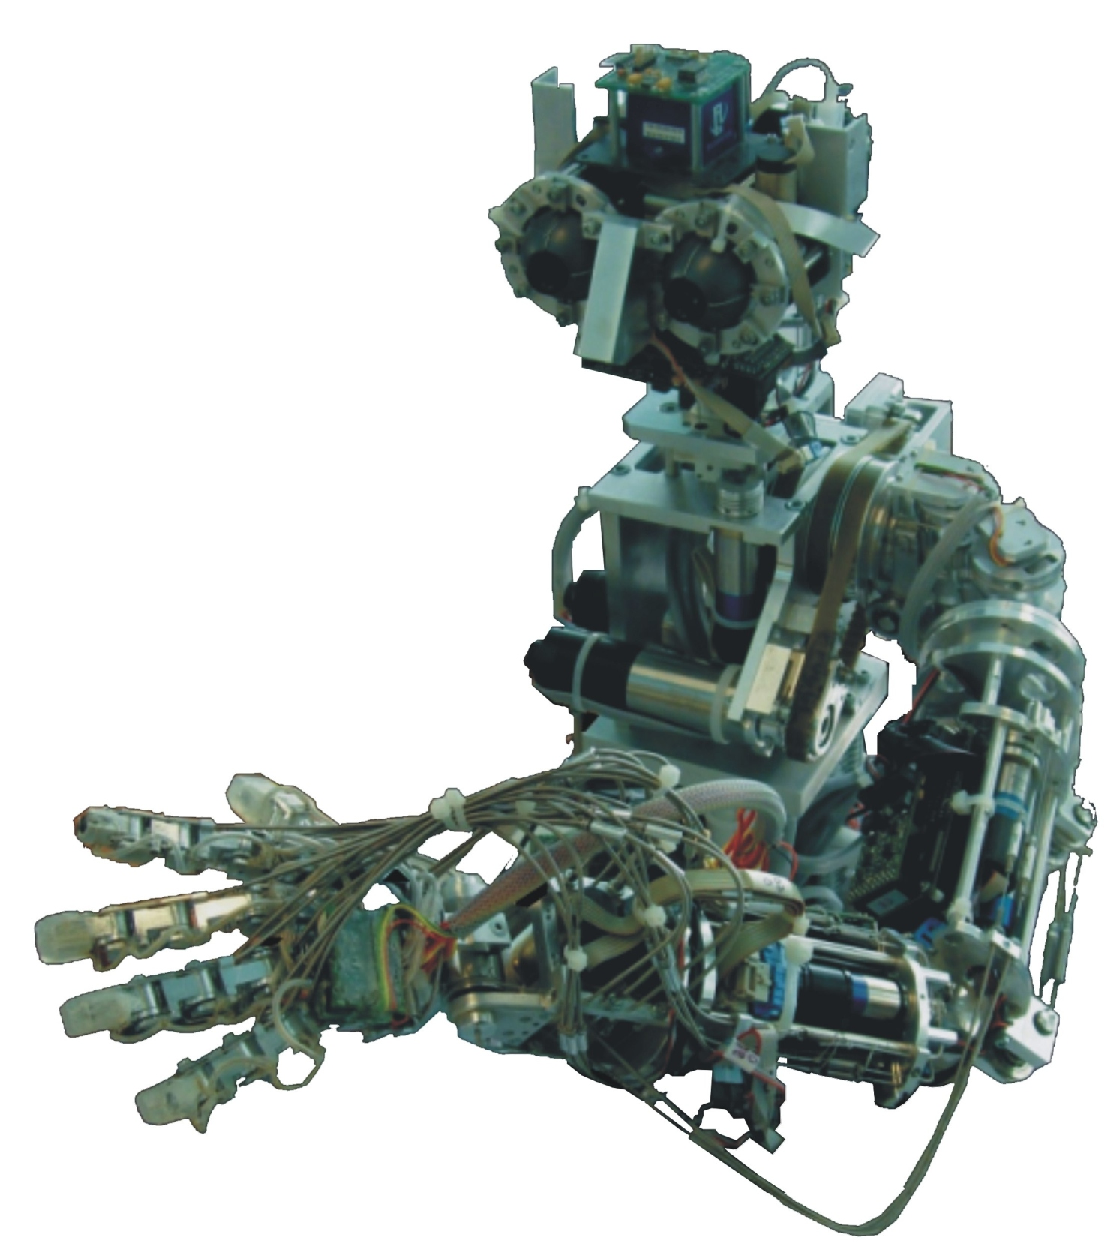
\includegraphics[width=2in]{imgs/james.ps}
\caption{James}
\label{figJames}
\end{figure}

\section{Method}\label{method}
As described in the introduction the ability to detect the hand of the robot, 
firstly presupposes the localization of regions that show alike and causal 
movement within the scene. For that we start by tracking all possible flocks 
of candidate regions in the image. Candidate regions are image patches of 
size $N \times N$ pixels that can be tracked well and where its containing 
features define a clear and unambiguous common direction. Concurrently to 
the tracking, the relative motion of the arm joints is recorded in order 
to have a base for comparing the visual information in the decisive step 
where all the visually gained trajectories are correlated with the arm joint. 

% ***********************************************************************************************
The ability to subsequently detect the hand of the robot, firstly presupposes the localization of regions that show alike and causal movement within the scene, as already introduced in section \ref{intro}. For that we start by tracking all possible flocks of candidate regions in order to determine which of the moving regions could be a part of the robot. Candidate regions are image patches of size $N \times N$ pixels that can be tracked well and where its containing features define a clear and unambiguous common direction. Concurrently to the tracking, the relative motion of the moving arm joint is recorded in order to have a base for comparing the visual information in the decisive step where all the visually gained trajectories are correlated with the single arm joint behaviour. 
%
%

% -----------------------------------------------------------------------------------------------
%
%																			localization - Assumptions
%
\subsection{Assumptions}\label{method:localization:assumptions}
% -----------------------------------------------------------------------------------------------

Proprioceptive feedback allows us a lot of information to exploit for various 
tasks. As soon as James generates motion with its arm as sort of 
self-exploratory motion generation it will cause changes in the visual and 
sensory perception. The robot senses a moving arm part which again indicates 
him to be attentive on visual feedback. \textit{Feeling} changes, means that 
there is the possibility to \textit{see} some changes which will then be 
correlated to the self-caused action behavior. At the current stage of 
development of this algorithm a few assumptions have to be set. The single 
arm joint motion

\begin{enumerate}
	\item produces enough net displacement in the plane parallel to the camera's CCD,
	\item takes place within the visual field of the robot's eye
	\item while James is neither moving its head nor its eye.
\end{enumerate}
In later stages of these works maybe all these constraints can be eliminated or at least incrementally eliminated.

Moving several joints at the same time or also moving different joints consecutively produces a complex movement in space (3D). This algorithm, however, is not yet using stereo vision. As a consequence of the missing dimension and the inexistence of a kinematic model of the arm (and rest of the body) it is not possible to calculate spatial motion out of two dimensional visual data. So, periodical waving or randomly moving one arm joint must mainly effect enough net displacement in a 2D plane parallel to the eyes' CCD element. 
To ensure this constraint an omnipotent criteria $ C_t $ is introduced that allows to move one single joint only, over an appropriate time interval. Looking back in the past at each time step using the standard deviation of the differences, ensures to transport the constraint over the whole interval, with a "safe" and short interrupt window.  In case of violation the algorithm starts newly or in an advanced stadium tries to localize the hand from the so far gathered information. We use the standard deviation to forgive the joints a possible change of the encoder values due to a shaking movement of another body part or joint. A shudder eventually causes a small peak in the time-elongation diagram of a joint $k$ that is thus robustly cushioned and not detected as intentional actuation.
%
We do not always receive stabilized images, even if the neck, head and eye actuators did not perform any active motion or somebody does walk somewhere through the scene, what in both cases could be understood as visible motion of the arm. Therefore the motion in the image has to exceed a certain motion threshold that is dependent on the focal of the eye's lens.
%
% -----------------------------------------------------------------------------------------------
%
%																						localization
%
\subsection{Localization}\label{method:localization}
% -----------------------------------------------------------------------------------------------
According to the approach, the attention system waits for a significant visual change in the scene. Due to the robot's ignorance of understanding the scene, any motion will be considered important that is greater than a certain amount. For a human being it is easy to make out and distinguish coherent and relevant regions. The following steps propose a possibility for the robot to do so as well.\\ \newline
%
% -----------------------------------------------------------------------------------------------
%
%\subsubsection{Classification of the optical flow}\label{method:localization:classification}
%\textbf{1) Classification of the optical flow}\newline%\label{method:localization:classification}
\textit{1) Classification of the optical flow}\\ \newline
% -----------------------------------------------------------------------------------------------
In order to localize regions that belong together, in sense of motion, we must first classify these regions and segment the global motion in the scene. Smaller regions that move together \textbf{within a larger neighbourhood } will later be put together into unique identifiable patches that contain several neighboured locations in the image moving equally and in the same direction.\\ \newline
%
% -----------------------------------------------------------------------------------------------
% 1
\textit{1.1: Motion computation}\\ \newline
% -----------------------------------------------------------------------------------------------
Between two consecutive time frames the motion is computed in a classical way where motion is computed by first selecting traceable points in the scene and then the displacement is calculated.
\begin{enumerate}
	\item \textit{Feature selection: } We pick a high number of good features, e.g.\ $n=1000$, to track and calculate for the selected number \textit{n} of features their position in the next image with the following step. A feature selection that is \textit{optimal by construction} for which tracking produces good results %not only for translational but also for affine motion 
	is the one proposed by J. Shi et. al\ \cite{GFT94-06}. %Using this technique assures a reliable choice for each type of motion.
	\item \textit{Feature tracking :} The pyramidal Lucas Kanade feature tracker searches in the image $I_t$ all features that were previously found \cite{PILKFT99} %. The Lukas Kanade tracker 
	and can be seen as a function that returns for each given feature in image $I_{t-1}$ the location in $I_{t}$ and receive $n$ displacement vectors; information that is describing the behaviour of the scene in the image.%\\ \newline
\end{enumerate}
%
% -----------------------------------------------------------------------------------------------
% 2
\textit{1.2: Representative patch displacement} \\ \newline
% -----------------------------------------------------------------------------------------------
As long as step 1.4 is unmet, the image is divided into a grid (step 1.2a)\ ) of equilateral patches where each optical flow is inserted and we start the classification process of the optic flow and decide on the regions belonging together. An object wandering through a scene projects in the image plane an area with an equivalent motion, thus this region is likely to own many optical flow vectors with similar or even equal values pointing to the same direction. Dividing the object's projection in the image plane into image patches must also divide the flow vectors into patches. These, into patches, summarized features are subregions that must still be moving like the corresponding object. \newline
On the other hand, if patches have already been initialized, the optical flow is placed in its corresponding patch (step 1.2b)\ ). \newline
%
% -----------------------------------------------------------------------------------------------
% 2a
%\paragraph{Step 3a): Initialization of the patches}\label{method:localization:classification:step3a}
\textit{a): Abstraction, initialization of the patches} \newline
% -----------------------------------------------------------------------------------------------
The result from the upper step 1), the current image, is first divided into a grid with $n_w \times n_h$ 2D patches where $n_w = \lfloor \frac{w}{N} \rfloor$, analogous for the height $n_h$, because $\vert \Lambda \vert = N \times N$ and the image size: $\vert I_{x,y} \vert = w \times h$. \newline
%Grid cells that eventually do not span the size of an ordinary patch are generously omitted, what means a maximal loss of the last $w \times (N-1)$ pixels in the height and the last $h \times (N-1)$ pixels in the width. Overall it does not make a big difference about the information content of the image. 
%Every patch $\Lambda_{F_k}$ covers in the initialization image cell \textit{i}, where the center of the patch \textit{(i,j)} is defined by:
%\begin{equation}
%\label{centering}
%center\left( \Lambda_{F_k} \right) =  \vec{c}_k\left( i, j \right) = \begin{pmatrix}i*N  + \frac{N}{2} \\ j*N  + \frac{N}{2}  \end{pmatrix}, \quad \forall i = 0 \ldots n_w \mbox{ and } \forall j=0\ldots n_h  \enspace .
%\end{equation}
%
% -----------------------------------------------------------------------------------------------
% 2b
%\paragraph{Step 3b): Assigning features (patching the flow):}\label{method:localization:classification:step3b}
\textit{b) Assigning features' flow to its patch} \newline
% -----------------------------------------------------------------------------------------------
Each feature is dropped into the cell according to its position. Consequently a patch $\Lambda_{F_k}$ absorbs all the displacement vectors that lie in the fixed patch size at the current position.\\
%:
%\begin{equation}
%\forall k = 1\ldots n: \quad center \left( \vec{d}_k \right)  =  center \left( \Lambda_{F_i}  \right),  \quad \mbox{where } \vec{u}_k \in \begin{bmatrix} c_x \pm \frac{N}{2} \\ c_y \pm \frac{N}{2} \end{bmatrix} \enspace .
%\end{equation}
%%
\begin{figure}
	\begin{center}
		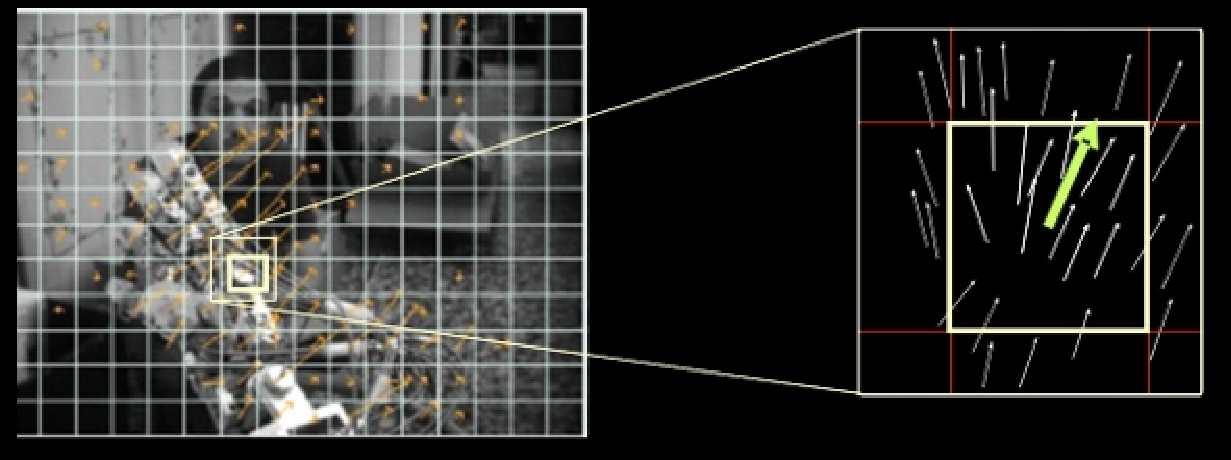
\includegraphics[width=3in]{imgs/method/step1to4.ps}
		\caption[Patching the flow. ]{\textbf{\textit{Patching the flow. Top left schematically shows an image extract with feature points and their displacements. As long as step 5 is not yet fulfilled, the image is subdivided into a grid of patches (top middle). Each cell in the grid assimilates all optical flow that is situated on its area (top right), however, if step 5 was satisfied and the tracking process is afoot, only relevant patches assimilate optical flow from newly determined features. The lower row illustrates step 4. }}}
		\label{fig:abstraction}
	\end{center}
\end{figure}
%
With this step the most important abstraction in the localization and detection process has been performed. Locations in the image array are decoupled from their original domain, the grey-level values (consult figure \ref{fig:abstraction} for the abstraction process). Our new informative system is a grid structure where each cell contains the correspondent set of displacement vectors $ \vec{d_i} \in \Lambda_k $ which are all centralized to the cell's center in respect to their start point. A set of loose values is not really classifying a small $ N \times N $ regions, much less larger regions. Likewise completely different displacement directions and amounts fall into the same $ \Lambda $ because the grid is placed over the image in a fix way, regardless the relationships in the scene.\\ \newline
%
% -----------------------------------------------------------------------------------------------
% 4
\textit{1.4: Representative patch displacement} \\ \newline
% -----------------------------------------------------------------------------------------------
After inserting all vectors in the patched image, for each patch the representative displacement is calculated. Each patch that has more than a certain amount of vectors greater than zero (that means traceable motion) are taken into account.
\begin{enumerate}
	\item \textit{Average angle}: In order to discard outliers in noisy regions and to tell the effective main direction of the patch, the angles must pass a corresponding confidence interval of the normal standard deviation of its comembers' values.
	\item \textit{General displacement vector}: Building the resultant (adding up the components) of the selected vectors leads to the common direction displacement of the patch.
\end{enumerate}
%
A reliable feature to classify the motion properties of the tracked image locations yields the direction component without building dependencies among the different $ \vec{v}_k = \vec{u}_k + \vec{d}_k $. Considering direction plus the velocity were building a strong unfoldable dependency for detecting these large regions. Apart from this fact, features sticking tight on a region that is spanning many patches, means an equivalent speed. So the velocity only differs in patches that lie on boarder regions of the object where there is anyway existing noise. The amount of the velocity is in neither of both directional classification cases an information with a qualitative statement, however, for the average displacement it matters. Additionally, due to the ratio between image size and patch size, where a single patch makes out at most approximately one per cent\footnote{In our set up $ percentage \left(  \Lambda, I \right) = \frac{N^2}{w*h}$ , where images have size 320 by 240 and $n < 20$ } of the whole image, the $ \vec{d}_k $ are assumed to be independently distributed  (in respect to their angle) at this point of time. We use the Gaussian distribution in order to determine a 90-percent confidence interval on the standard deviation of the angular values respective to the average angle of all $\vec{d}_k $ to eliminate the gross outliers. In figure \ref{fig:abstraction} we schematically sketched the representative displacement vector $\overline{\vec{d}_k}$ of patch $k$. Let us denote a set $\mathcal{A}$ that accommodates all $\vec{d}_i \in \Lambda_k$ that pass the 90-percent interval.% in equation \ref{confint}. 
Noisy regions are likely to be disqualified already here, otherwise at the next steps. Patches without any displacement logically go into the discard. 
\begin{equation}
	\alpha_{d_i} = \arctan{ \left( \frac{d_{i,y} }{d_{i,x} } \right)}, \quad \mbox{where } \forall \vec{d}_i \in \Lambda_{k} , i=0 \ldots n_{d_k} \enspace .
\end{equation} 

Building the average and standard deviation on the angles:
\begin{equation}
\label{alg:avg}
\overline{\alpha}_{d_k} = \overline{ \alpha } \left( \Lambda_k \right)  = \frac{1}{n_{d_k}} \sum_{i=0}^{n_{d_k}-1} \alpha_{d_i} \enspace .
\end{equation}
%
\begin{equation}
\label{alg:std}
\sigma_{d_k} \approx \sqrt{ \frac{1}{n_{d_k} - 1} \sum_{d_i \in \Lambda_k} \left[ \left( \alpha_{d_i} - \overline{ \alpha}_{d_k} \right) ^2\right] } \enspace .
\end{equation}
%
With equation \ref{alg:avg} and \ref{alg:std} the 90-percent confidence interval and t as the $95^{th}$ percentile of the Gaussian distribution, where $\Pr\left(-t<A<t\right)=0.9$, is defined as follows:
%
\begin{equation}
\label{confint}
\begin{bmatrix}  \overline{ \alpha}_{d_i} - \dfrac{t*\sigma_{d_k}}{\sqrt {n_{d_k}} } \end{bmatrix} 
\leq \alpha_{d_i} \leq 
\begin{bmatrix} \overline{ \alpha}_{d_i} + \dfrac{t*\sigma_{d_k}}{\sqrt {n_{d_k}} } \end{bmatrix} \enspace .
\end{equation}
%
Finally all $|\mathcal{A}|$ displacement vectors whose angles passed the 90-percent interval are building a resultant that depicts the representative displacement for that patch:
%
\begin{equation}
\label{representative}
\overline{ \vec{d_k }} =  \sum_{j \in \mathcal{A}}{\frac{\vec{d}_j}{|\mathcal{A}|} } \enspace .
\end{equation}
\\ \newline
%
% -----------------------------------------------------------------------------------------------
% 4
\textit{1.4: Classification - Flocking / Classification of the patches and building flocks} \\ \newline
% -----------------------------------------------------------------------------------------------
As long as this step did not succeed in a satisfying manner or is performed the first time the following classification step must be executed. For each patch $i$ with an angular value its eight neighbours are inspected to decide if the patch shall be marked for tracking. 
\begin{figure}
	\begin{center}
		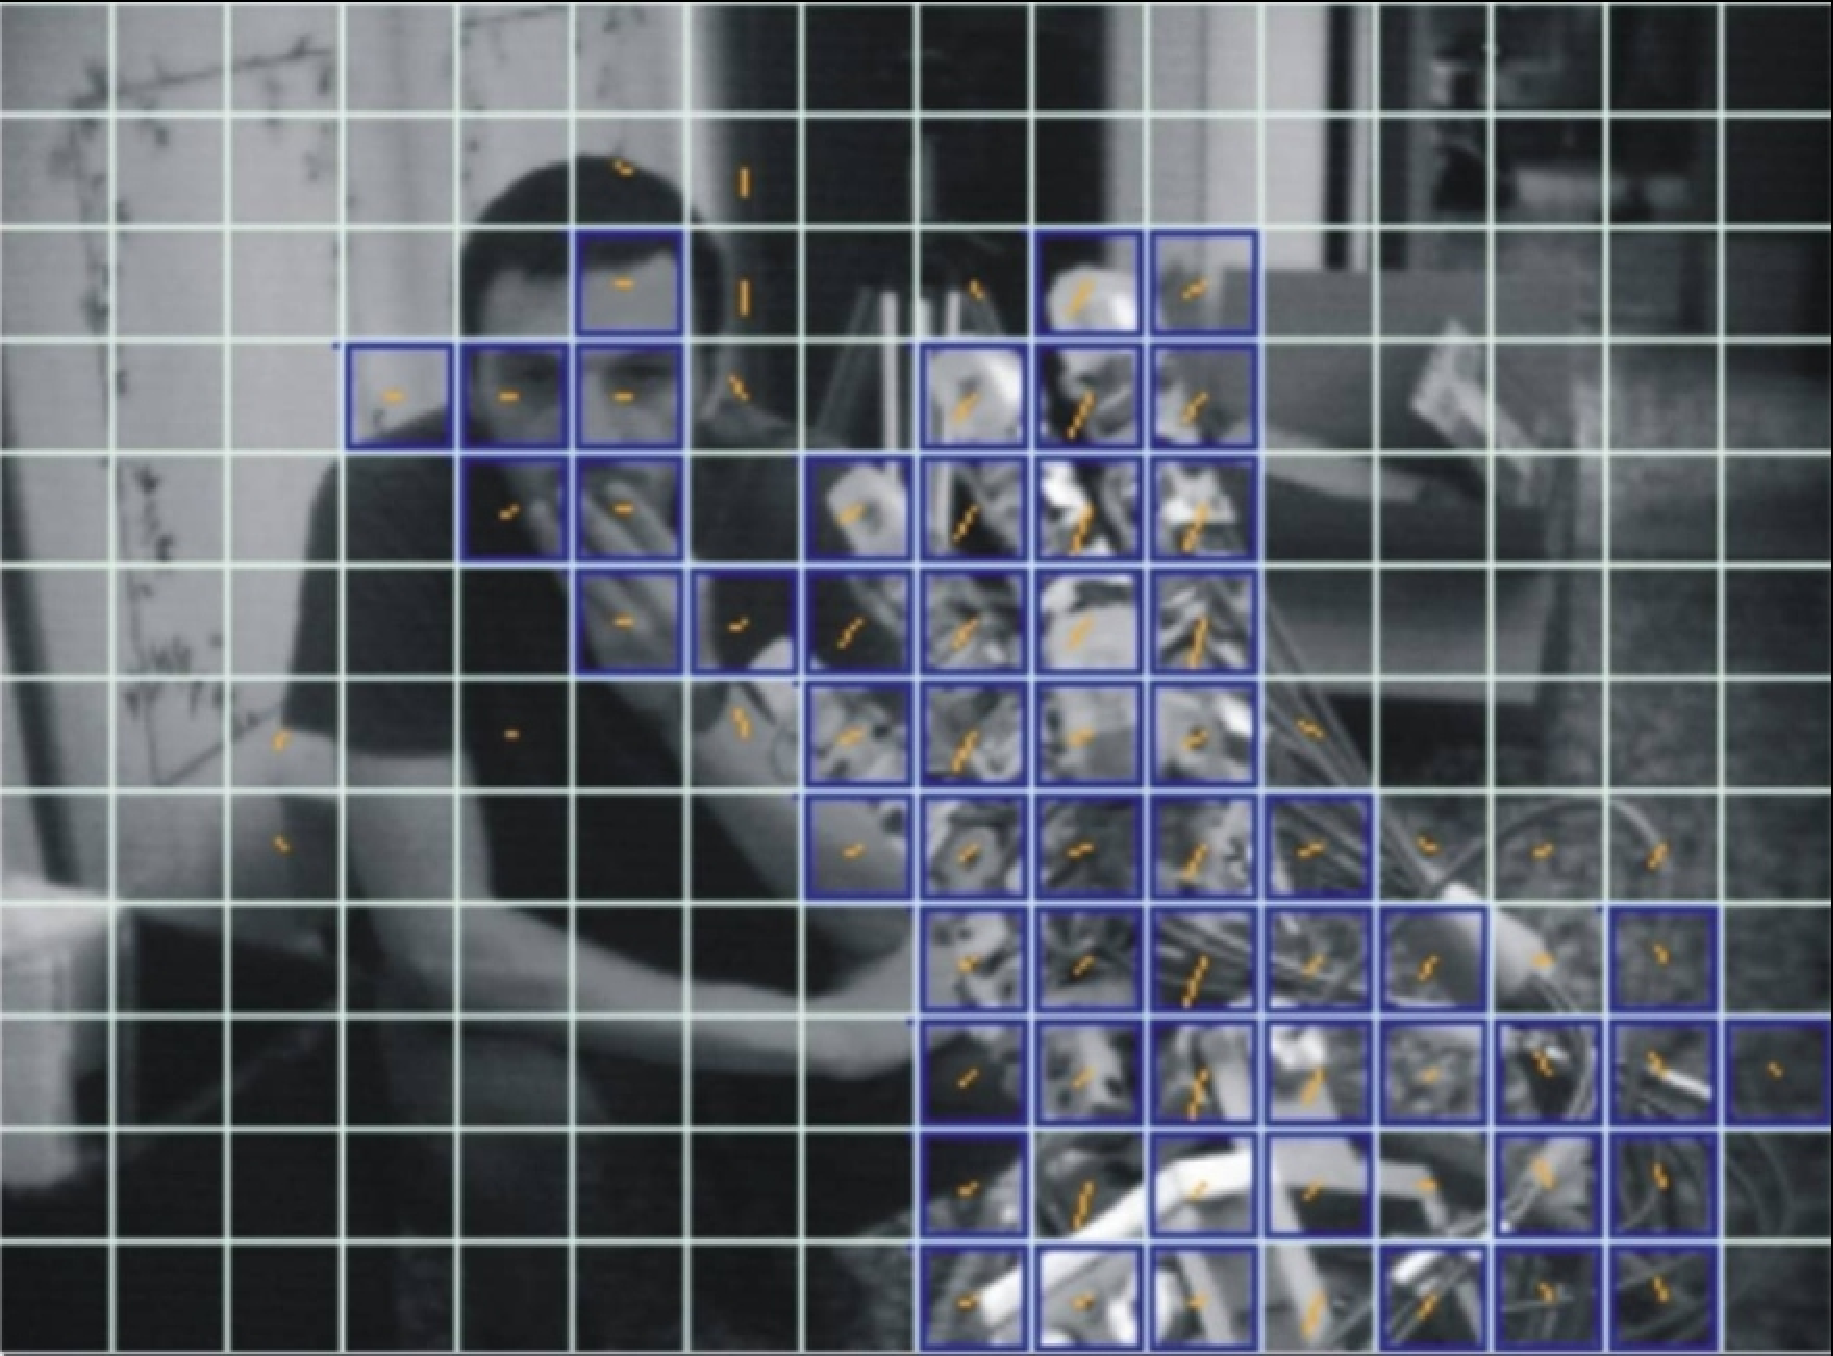
\includegraphics[width=2in]{imgs/method/selection.ps}
		\caption[Feature patch grouping. ]{Feature patch grouping. For each patch in the grid the neighbours are contemplated. If a patch has more neighbours than a minimal threshold $\rho_{MIN\_NEIGHBOURS}$ fulfilling that their direction in motion is lying between $\pm \beta_{range}$, it is marked as a relevant patch. As this process continues in the end we have flocks of patches that cover a bigger region moving in the same way, what can be seen as visual grouping according to \cite{ULGII23} }
		\label{fig:flocking}
	\end{center}
\end{figure}
%
A new threshold $\rho_{flow}$ ensures that not single patches or too small areas will be tracked, thus one single patch, e.g.\ with the size of $13 \times 13$, with no neighbour-patches is unlikely to depict a ``bigger'' region. A perfect coverage of the whole objects would be nice, but hardly possible to achieve. Reasons are the limited amount of features that are not equivalently distributed over all moving object, or that an object's surface is simply not have enough well traceable features. The aggregation of single patches to larger and distinct flocks of patches with "equidirectionally" motion among each other %is likely to happen 
turns up the for different objects with different motion trajectories. Coherent patches show a sufficiently equivalent direction compared to its neighbour according to a predefined aperture angle window. All patches that have more than a number of directly adjacent patches with the same behaviour, e.g. two out of an 8-neighbourhood in our setup, satisfying  $\beta_{range}$ get an unique identity and are kept for tracking.
% The just performed flocking of patches, again, does not necessarily cover a single object, but all the moving objects satisfying the above qualifications.	So, technically speaking for every patch $i$ with an angular value its eight neighbours are inspected to decide if the patch will be marked for tracking, see illustration in figure \ref{fig:flocking}. This importance measure is calculated by visiting all 8 neighbours according to the following scheme: \\
If the patch has a neighbour lying within an angular range (e.g +/-25 degrees) of the start patch's average angle, the neighbour patch is assumed to belong to the same region and therefore increases the importance measure of patch $i$ (see equation \ref{neighbours}). One patch can have at most eight neighbours pointing to the same direction. \\
%As we visit each grid cell on the patch image and determine the importance for tracking this cell we discard regions that remain alone or are not interesting to track. Obviously several flocks of patches with different values can be passed for tracking; where as each flock denotes a huge set of pixels that are very likely to move \textit{together} and belong to any moving object in the image fulfilling all conditions till this point.
%%
%\begin{equation}
%\label{neighbours}
%	neighbours\left( \Lambda_k\right) \ = \sum_{j=1}^{8} \omega_{kj}, 
%	\quad \mbox{ where } \omega_{kj} = 
%	\begin{cases}
%		1, & \mbox{if } 
%			\vert \overline{\alpha}_k  - \overline{\alpha} \left( neighbour \left( \Lambda_k, j \right) \right) \vert \leq \beta_{range} \\ 
%		0, & \mbox{else. } 
%	\end{cases}
%\enspace .
%\end{equation}
%The set $Q$ of patches that get qualified, due to their neighbour-relationships, is defined by:
%\begin{equation}
%\label{qualify}
%	Q\ = \left\lbrace \left( \Lambda_k \right): neighbours\left( \Lambda_k\right)  \geq \rho_{MIN\_NEIGHBOURS} \right\rbrace \enspace .
%\end{equation}
%In other words, the set of all patches (the entire image) will be divided in two disjoint sets such that: $I \left( t\right) = Q \cup \overline{Q}$ and $Q \cap \overline{Q} = \emptyset$.
%%
%Similar to the previous step, where the overall motion in the image must be higher than threshold $\rho_{motion}$, the overall percentage of selected patches must exceed $\rho_{flow}$ so that condition 
%\[
%C3: \quad \dfrac{\vert Q \vert}{\vert Q \vert + \vert \overline{Q} \vert} > \rho_{flow} \enspace .
%\]
%%
In other words, the set of all patches (the entire image) will be divided in two disjoint sets such that: $I \left( t\right) = Q \cup \overline{Q}$ and $Q \cap \overline{Q} = \emptyset$.
As long as this threshold is not fulfilled the whole procedure `%(all steps of 2)
 is continuously repeated. The example in figure \ref{fig:classified} shows the flocked regions, the head and the robot's hand. 
%
%\begin{figure}[H]
%	\begin{center}
%		\includegraphics[width=.90\textwidth]{data/images/halo/classified.jpg}
%		\caption[Grouped features worth to track. ]{Grouped features worth to track. Two images of a sequence that show in what fulfilling all conditions until step 3 result into; on the left hand side the binarized image difference from I(t) and I(t-1) and their optical flow }
%		\label{fig:classified}
%	\end{center}
%\end{figure}
%
\\ \newline
%
% -----------------------------------------------------------------------------------------------
%
\textit{2) Tracking}\\ \newline
% -----------------------------------------------------------------------------------------------
% 6
By the time the classification provides one or several flocks marked as important regions in the scene, the tracking process launches. At each point in time the displacement of each identifiable patch is recorded, where steps 1 to 4 supply the tracker with the needed information. But as we later want to close the action-perception loop, we also have record the yet independent body sensory information, the encoder values. By the time tracking started the procedure lasts over a time window $\tau_{tracking}$, e.g.\ 200 frames.
%
As this localization problem cannot be solved by pure vision, the motor encoder values are tracked as well as the patches that have been qualified for tracking in the previous steps. Therefore tracking consists of ``tracking'' two different perception inputs.
% -----------------------------------------------------------------------------------------------
% 2
\textit{2.1: Classification - Flocking / Classification of the patches and building flocks} \\ \newline
% -----------------------------------------------------------------------------------------------

\paragraph{Step 6: Tracking visual information:}
%
Let us assume that the initialization phase completed at $t_{ready} -1$ and tracking can be started. Set $Q$ contains a fixed number of patches that are qualified for tracking and each patch has an own identification (ID). Identification is a basic need in order to decide which of the tracked patches, are the patches lying on the hand in the last step of the localization process (step 7). All good features to track chosen for at $t-1$ and their optical flow tell where these features are to find in the current image. The newly achieved displacement vectors do either fall into one of the patches $\in Q$ or are lost in the irrelevant space. Patches are then treated as in steps 3b and 4 from where the next displacement vector results. The patches from $t-1$ break out of their grid structure, perform their first step and move to their new position according to the displacement. From point in time $t=t_{ready}$, the essential part of the algorithm starts and tracks all $\Lambda_{k \in Q} $ for a time window $\tau_{tracking}$. As long as the time window has not been interrupted, due to the restrictive condition $C_t$, or terminated, steps 1 to 4 are repeatedly performed. The new center of a patch at $t$ is:
%
\begin{equation}\label{newpos1}
	\vec{c}_k\left( t \right) = \vec{c}_k \left( t -1 \right) + \vec{d}_k\left( t -1, t\right) \enspace .
\end{equation}

For the duration of tracking, each position of a patch in the image is the resultant of all the past $c_k$s. Building at each time step the length of the difference vector between the start position of a patch and the current position, we generate a motion graph - the trajectory. Please see figure \ref{fig:tracking} where tracking is shown for one possible sequence.
Basic idea is that the feature-populated hand shifts in the image plane also causes to shift the features lying on the hand. As the displacement is not infinitively big, but rather small and due to the fact that patches follow textured region, it is likely that new features fall again into those patches. But as tracking by this method is an averaging method over a certain piece of the image and its feature, it is possible that a $\Lambda_{ID\left( k \right) } \in Q$ is not fast enough to follow the ``object'' it originally was attached to. For instance, if a border region loses one feature after another until it stops, unless not being picked up again. As our aim is to track the hand, we assume that the hand will never be hidden or occluded by another object, otherwise continuous trajectories can not be reasonably built and avoid as much as possible previous cases.  The patches would be drawn away, because features are independently chosen from its predecessor features for every frame with which we ensure that features remain independent and always contemplate only important - textured - regions (that are easy to track). In the end the trajectories of some patches that did not stick on the hand and will not be correlating with the hand. On the other hand, if there have been chosen features on the robot's hand, they will likely been chosen in the next frame, consequently remain on the hand. We can also show and ensure that this method is robust to behaviour where the object is resting and producing no (visible) action. This is how the markerless tracking works, in section \ref{results} we will show the results, where different windows sizes and different environments show that this algorithm is reliable under difficult circumstances. 

For each patch there is built one characteristic trajectory $ \Phi_{\Lambda_Q} $ as a function of time. Figure \ref{fig:visualtrajectory} shows possible visual trajectories, gained with equation \ref{trajectory}. Again, the trajectory describes the relative disposal history of a patch over time from its origin in the grid where the patch had been instantiated. Each time step stands for a spatial elongation \textit{e} from its origin. Recording this elongation as function of time enable us to compare the visually gained trajectories with the motor joint trajectory. 
%
$\forall \Lambda_i \in Q \mbox{ and } t \geq \left( t_{ready} -1\right) :   $
\begin{equation}
\label{trajectory}
	\Phi_{\Lambda_{i}, e_{xy}} \left( t \right) = \sqrt { \left( { \vec{c}_{ \Lambda_{i} , x } \left( t_{ready} -1 \right) - \vec{c}_{\Lambda_{i} , x} \left( t \right)} \right)^2 +  \left( \vec{c}_{\Lambda_{i} , y} \left( t_{ready} -1 \right) - \vec{c}_{\Lambda_{i} , y}\left( t \right) \right)^2} \enspace ,
\end{equation} 
$\mbox{and } \quad \Phi_{\Lambda_i , x,y} \left( 0 \right) = \vec{c}_{\Lambda_i} \left( t_{ready} -1 \right) \enspace .$
%
%
%\begin{figure}[ht]
%	\begin{center}
%		\includegraphics[width=1.0\textwidth]{data/images/halo/visualtrajectories.jpg}
%		\caption{ Trajectories created by tracking patches over a timewindow $\tau_{tracking}$. }
%		\label{fig:visualtrajectory}
%	\end{center}
%\end{figure}
%
%
\paragraph{Step 6: Tracking encoder values:}
\label{halose:halo:algorithm:step8enc}
%
The changes of the encoder values - motor-sensory perception - contain same temporal displacement information like the visual trajectories, if they caused the change. The relative changes of the actuated joint are recorded similar to the patch motion.  Encoder trajectories are built by the difference of the relative angular value in respect to its angular value at the start $t_0 = t_{ready}-1$, see green trajectory e.g. in figure \ref{fig:corr}. Our assumptions, that the effected changes are visible and only one joint is moving, ensure that there exist visual and joint trajectories with a very similar behaviour. O%f course, a quanyative statement about absolute elongation or the absolute direction is not possible - just about the (relative) behaviour. 
Motor joint trajectories are built according to: 
\begin{equation}
\label{jointtrajectory}
	\Phi_{q_{k}, e_{\alpha}} \left(t\right) = \left| \left( \alpha_{q_{k}} \left(t\right) - \alpha_{q_{k}} \left(t_0-1\right)\right) \right| \enspace .
\end{equation} 
%
%
%\newpage

	
	
% -----------------------------------------------------------------------------------------------
%
\textit{1) Tracking}\\ \newline
% -----------------------------------------------------------------------------------------------
	% 7
\textit{Localization}: At this point the most important step, the conclusion of all previous steps takes place. The 						robot differentiates between the experience of its body movements and other moving entities in the environment, see 				\cite{FLSAUEL03-02}. The step from \textit{confusion} to level 1 of self-awareness, \textit{differentiation}, is 							taken by correlating the visually gained information with the bodily experience. Technically, the set of tracked  						patches are confronted with the encoder values. Each patch trajectory that highly correlates with the joint 									trajectory is now qualified to be part of the robot and denotes a region in the image plane where the hand stays, from where in the segmentation part the hand will be extracted from its environment.
\\ \newline
%
%
% -----------------------------------------------------------------------------------------------
%
%																						detection
%
\subsection{Detection}\label{method:detection}
% -----------------------------------------------------------------------------------------------
% 8
\textit{Segmentation}: During tracking we temporary saved the images and use them to retrieve the background with the method described earlier in \ref{methods:bics}. From image $I_{loc}=I_{ready + \tau_{tracking}}$, where the hand had been localized, the background  is subtracted to retrieve the foreground from the region of interest found by step 7.

%
The algorithm, seen as a complete entity, is a surveillance of the visual scene over a certain period of time with a simultaneous processing of visual and proprioceptive information. It can be described as model consisting of a 3D array $V_{x,y,t}=I_x\ \times\ I_y\ \times\ I_t$ of visual information\footnote{where $I_x,I_y,I_t$ denote sets of indices, analogous the upcoming notation for the arm joints} (practically a video sequence), a 2D array $S_{q,t} = J_k \times J_t$ of motor sensory feedback and set of functions. 

The visual basis for each timestamp is a grayscale image $I$ described by a 2D set of pixel values, where $I(\vec{x})=I(x,y)$ defines the grayscale value at the location $\vec{x}=\left[x\ y\right]^T$. The image has a size of $w \times h$ pixels. 
For each point in time $t$ the joints vector $\vec{q} = \left[ q_{0}\ q_1\ \ldots\ q_{K-1} \right]^T$ represents the relative angle position (displacement in degree angles) of the $k$ arm encoders in respect to the time before. %, where $q_k$ denotes one of $K$ joints. %In case of James the cardinality $\left|\vec{q}\right|= 15$, resulting from 7 arm and 8 hand joints.

For further proceedings a 2D structure called image patch $\Lambda$ takes up an important role. In our case a 2D patch is actually a 3D array with a \textit{single temporal} index and denotes a \textit{spatial} $N \times N$ neighbour\-hood of pixels: $\Lambda_t = \left\{I_x\ \times\ I_y\right\}\ \times\ \left\{t\right\} = \left(\Lambda, t\right)$.



%**********************************************
\subsubsection{Localization - Mapping and Identification}
\label{halose:halo:algorithm:localization}
%
\paragraph{Step 7: Localization of the hand}
\label{halose:halo:algorithm:step7}
%
The localization process actually started with the beginning of this algorithm, however, the most important step to localization happens here in step 7. All the collected information, more precisely the vision trajectories, must now be correlated with the encoder trajectory. For each patch trajectory confrontation, we calculate the correlation coefficient using the standard deviation, analog to equation \ref{alg:std}, and the empirical covariance:

% * This method returns the empirical covariance of a two-dim test series stored in a bottle of n double values.
% * s_xy =  1/(n-1) * Sum[ (x_i - x_)(y_i - y_) ] 
% *
\begin{equation}
\label{covariance}
	cov_{\Phi_{\Lambda_{i}, e_{xy}}, \phi_{q_{k}, e_{\alpha}}} = \frac{1}{\tau_{tracking}-1} * \sum \left[  \left(e_{xy}\left(t\right) - \overline{e}_{xy} \right) \left(e_{\alpha}\left(t\right) - \overline{e}_{\alpha}  \right) \right] \enspace ,
\end{equation}
what then is used in:
%
% * r =  s_xy / (s_x*s_y)
% *
\begin{equation}
\label{correlation}
corr_{\Phi_{\Lambda_{i}, e_{xy}}, \phi_{q_{k}, e_{\alpha}}} = \frac{cov_{\Phi_{\Lambda_{i}, e_{xy}}, \Phi_{q_{k}, e_{\alpha}}}}{ \sigma_{\Phi_{\Lambda_{i}, e_{xy}}} * \sigma_{\Phi_{q_{k}, e_{\alpha}}}} \enspace .
\end{equation}

The correlation qualifies every patch that responded in a cooperative manner bigger than a elimination procedure thresholded by $\rho_{corr}$ returns the set of those patches lying with a very high probability on the hand. This end set $\Omega$ can be described by:
%
\begin{equation}
\label{endset}
 \Omega = \left\lbrace \left( \Lambda_{k \in Q} \right): corr_{\Phi_{\Lambda_{i}, e_{xy}}, \phi_{q_{k}, e_{\alpha}}} > \rho_{corr} \right\rbrace \enspace .
\end{equation}
%
\begin{figure}[h]
	\begin{center}
		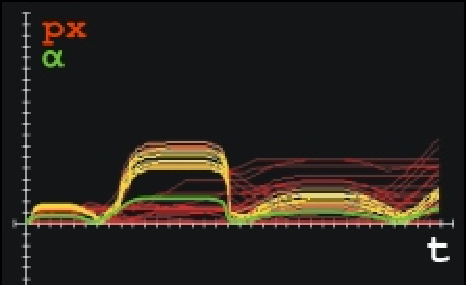
\includegraphics[width=3.5in]{imgs/method/correlation.ps}
		\caption[Trajectories correlating with the behaviour of the arm. ]{Trajectories correlating with the behaviour of the arm. All tracking trajectories of the qualified patches over time are red unless they do not match with the green motor joint trajectory and become yellow. On the left hand side we see an example with a positive result, on the right hand side obviously a negative.}
		\label{fig:corr}
	\end{center}
\end{figure}
%
In figure \ref{fig:corr} two different data sets are shown, where in the left set of trajectories there have been found patches matching to the self-actuated motion, on the other hand in the right hand non of the patches fit. $\rho_{corr}$ is adaptable, but experience show, later in \ref{results}, that under whatever conditions a range from 0.9 up to 0.97 are good thresholds. In figure \ref{fig:example} an experiment result is shown, where the patches $\in Q$ are displayed. The white circles (see image in the middle of figure \ref{fig:example}) denote the patches that are identified by the robot as patches following its motion.
%
%\begin{figure}[ht]
%	\begin{center}
%		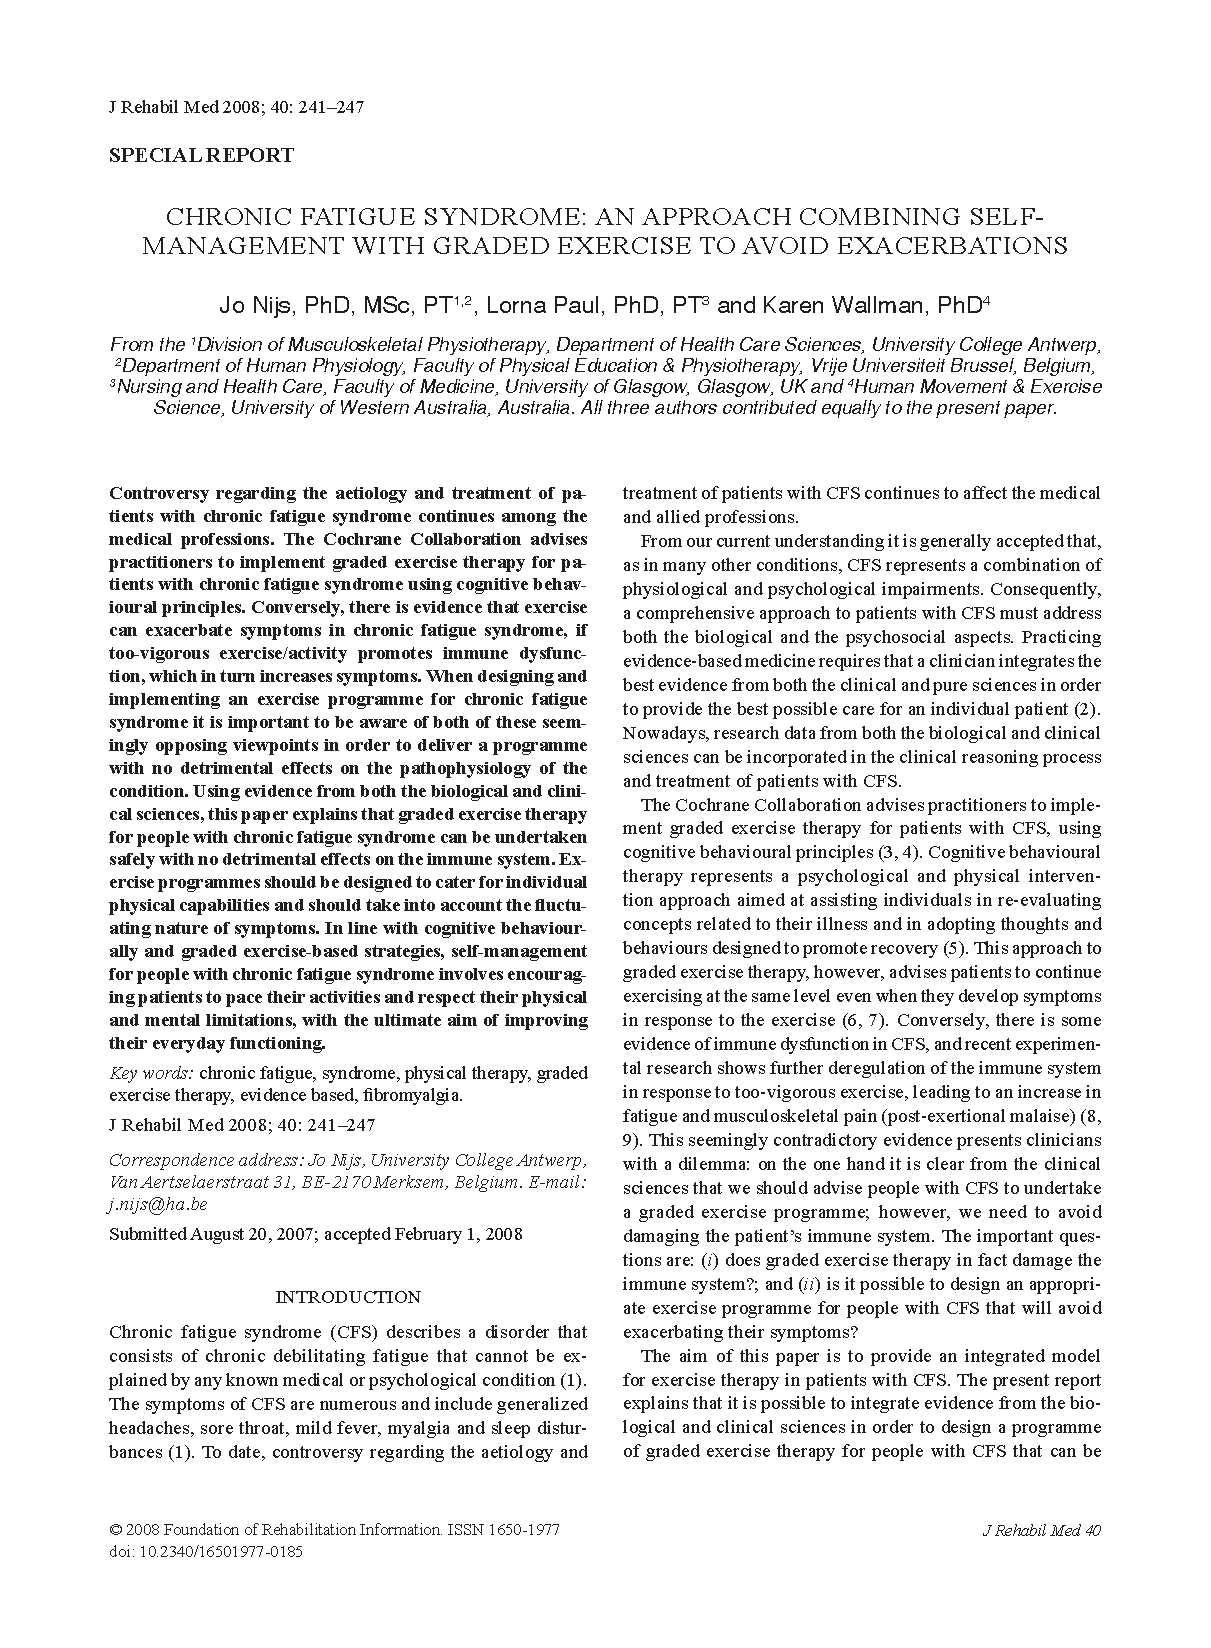
\includegraphics[width=.90\textwidth]{data/images/halo/example.jpg}
%		\caption[Hand localization of aperiodic arm motion. ]{Hand localization of aperiodic arm motion. In this example an aperiodic movement of the forearm generates the following result of the hand localization. On the most right (top), the selected region is elucidated by applying the convex hull over the resulting patch locations. Above we ``masked'' the ROI to explicitly show the reader the interesting region. }
%		\label{fig:example}
%	\end{center}
%\end{figure}
%
The patches correlating with the robot's actuated motion define a region of interest (ROI) where the hand is apparent. The convex hull around the selected patches is a way to mark the chosen ``hand'' area. Marking the ROI is as an intermediate step for the reader to understand how far we came with the localization, consult figure \ref{fig:roi}. The next step will segment the hand from this area.
%
%\begin{figure}[h]
%	\begin{center}
%		\includegraphics[width=.90\textwidth]{data/images/halo/roi.jpg}
%		\caption[Localized region of the hand. ]{Localized region of the hand. The region of interest is marked with the convex hull of the selected patches and denotes the location of the hand.  }
%		\label{fig:roi}
%	\end{center}
%\end{figure}
%
% -----------------------------------------------------------------------------------------------
%
%																						detection
%
\subsection{Detection (Segmentation)}\label{method:detection}
% -----------------------------------------------------------------------------------------------
Segmenting information means to extract or classify the one information, that we are interested in, from other ``useless'' information. In this particular case, the localization process returns a region of interest (ROI), see figure \ref{fig:example} on the outer right, denoted as the area where the hand, or parts of it, appear in the visive field. As we were not tracking (single) pixels from the hand but regions of ``equidirectional'' motion, we do not have the possibility to extract the hand. Still it is unclear how the hand looks like. The ROI contains the information about the hand, but unfortunately also parts of the environment.

The perfect way to extract all (moving) objects in front of a stationary scenery, is to subtract the \textit{known} background, seen in image \ref{fig:segmentation}. Explicitly we stress on the property: known background. But as we know a robot may act in different environments and e.g.\ moves its head, the background is not always the same and is rather a temporal constraint. The ROI defines a spatial window, which, observed over time, provides information for recovering the background. For recovering the background using the by-gone times A. Colombari et al.\ proposed a technique, described in section \ref{methods:bics}. Assuming that we can recover the background perfectly, an exact segmentation of the hand, or an excerpt of it limited by the ROI, is possible (see figure \ref{fig:perfsegm}). The visual model of the hand, given by the exact segmentation, provides the used information for later visually guide the robot's own hand in a reaching process.
%
\begin{figure}[h]
	\begin{center}
		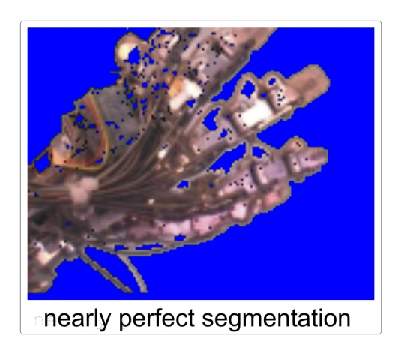
\includegraphics[width=3.5in]{imgs/method/perfsegm.ps}
	\end{center}
		\caption[Segmented hand. ]{Segmented hand. A nearly perfect segmentation of the hand extract gained by image $I_{t_{ready}+\tau_{tracking}}$ and the background gained with BICS, see page \pageref{methods:bics}.}
		\label{fig:perfsegm}
\end{figure}
%
\paragraph{Step 8: Segmentation:}
\label{halose:se8}
% 
At time $t_{ready}+ \tau_{tracking}$ we localized the hand. On the basis of the patches that were classified as part of the robot, we build a bounding box around the region of interest. Minimizing the area around the hand, enables to reduce the computing cost for retrieving the background and to increase the probability to extract only the hand and not other objects from the foreground. As above mentioned, we extract this bounding box from all the past images to recover the background. Once the background is computed, the foreground is a pixel-wise subtraction of the background from the region of interest. The values of the difference are binarized with a threshold, we used the same as in equation \ref{eq:bics:bindiff}. The binarization returns a mask, which is then applied on the image containing the extracted ROI and clearing the uninteresting (background) pixels. The procedure is illustrated in figure \ref{fig:segmentation}.
%
\begin{figure}[ht]
	\begin{center}
		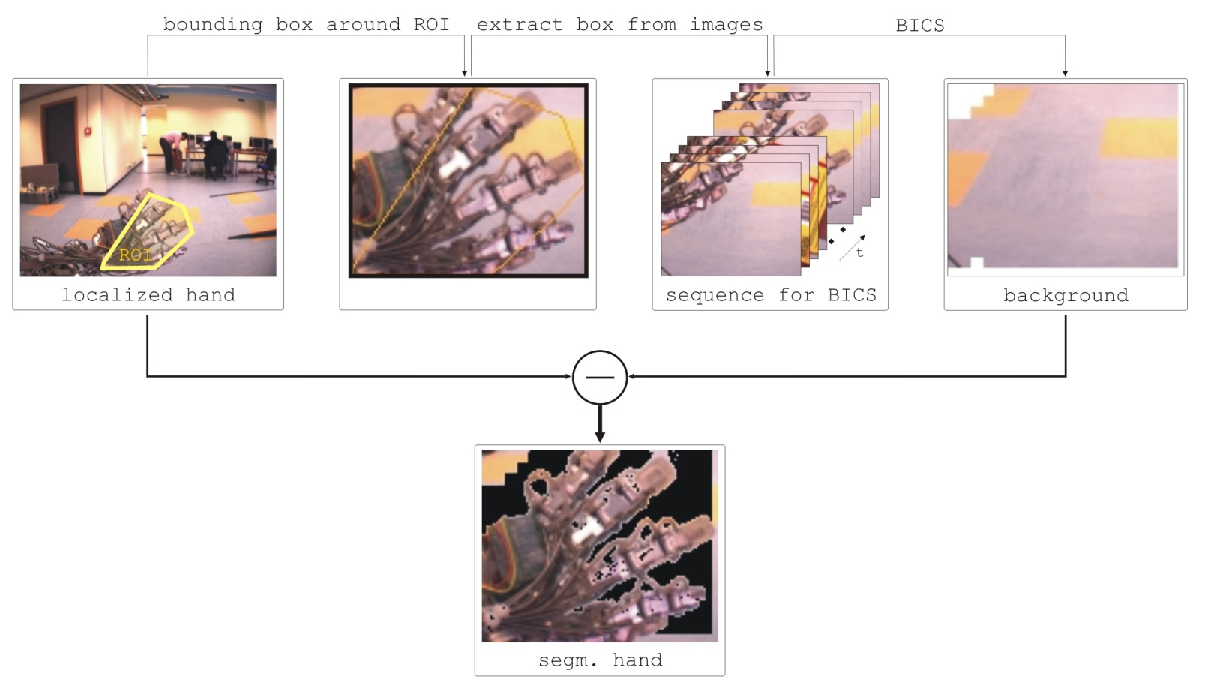
\includegraphics[width=3.5in]{imgs/method/segmentation.ps}
	\end{center}
		\caption[Detection procedure. ]{Detection procedure. At point in time $t_{ready}+ \tau_{tracking}$ we extract the bounding boxes from all images we the hand was localized. With the BICS algorithm the background is recovered. Finally the background is subtracted from the original image where the hand lies. Decision on the pixel differences is made on binarizing the values.}
		\label{fig:segmentation}
\end{figure}
%
\subsubsection{BICS}
\subsubsection{Problem}

\section{Results}
\label{sec:results}

In this section we report the results of the experiments we carried out
to quantify the performance of the reaching movements. Following the proposed strategy, 
in order to reach for the 
target we first need to fixate it, i.e. $\utarget = 0$. Using the available sensor (i.e. vision) the best we can do to precisely reach the target is moving the hand to the fixation point, i.e. $
{\uhand} \longrightarrow 0$. Clearly, the image plane distance $\| \uhand - \utarget \|$ can be used as a rough estimate of the reaching precision, i.e. of the Cartesian distance between the target to be reached and the position of the hand. Specifically, assuming infinite resolution of the camera sensor, if $\| \uhand - \utarget\| = 0$ then the hand has exactly reached the target.

\subsection{Open Loop}
The first attempt to reach the target consists in using the learned forward model 
(\ref{Eq:forward}) and the strategy (\ref{Eq:reaching2})
to choose the arm configuration $\q_{arm}$ which brings the hand to the center 
of the image planes. Clearly, if the forward 
kinematic function (\ref{Eq:forward}) were perfectly represented and if the target were reachable, then we would have 
$\mathbf x_{hand} =  \mathbf x_{target}$, which implies that the target-hand Cartesian distance 
 is zero (see Section \ref{sec:reaching} for details). Therefore, in this ideal case, the open loop 
 strategy already results in $\| \uhand - \utarget \| = 0$. In practice, the model 
 (\ref{Eq:forward}) cannot exactly represent the system's kinematic\footnote{Part of the representational 
 errors are related to the representation of the kinematic function, in this case the
 so called Receptive Field Weighted Regression model. Part are due to the mechanical plays and backlash of the
 mechanical structure.}. Therefore, even tough we can find $\q_{arm}$ such that $\mathbf x_{hand}=
 \hat f_{arm}(\mathbf q_{arm})$ it is not guaranteed that after the movement execution 
 $\| \uhand - \utarget \| = 0$. Figure \ref{Fig:ImagePlaneOpenLoopErrors}
 shows the image plane errors after the execution of the open loop movement. The plot has been obtained
 by fixating a target and performing a series of open loop movements. Each open loop
 movement was different because (\ref{Eq:reaching2}) was solved 
 by choosing a different value $q_{20}$. 


\begin{figure}
  % Requires \usepackage{graphicx}
  \begin{center}
	\begin{tabular}{ccc}
	  \parbox{30mm}{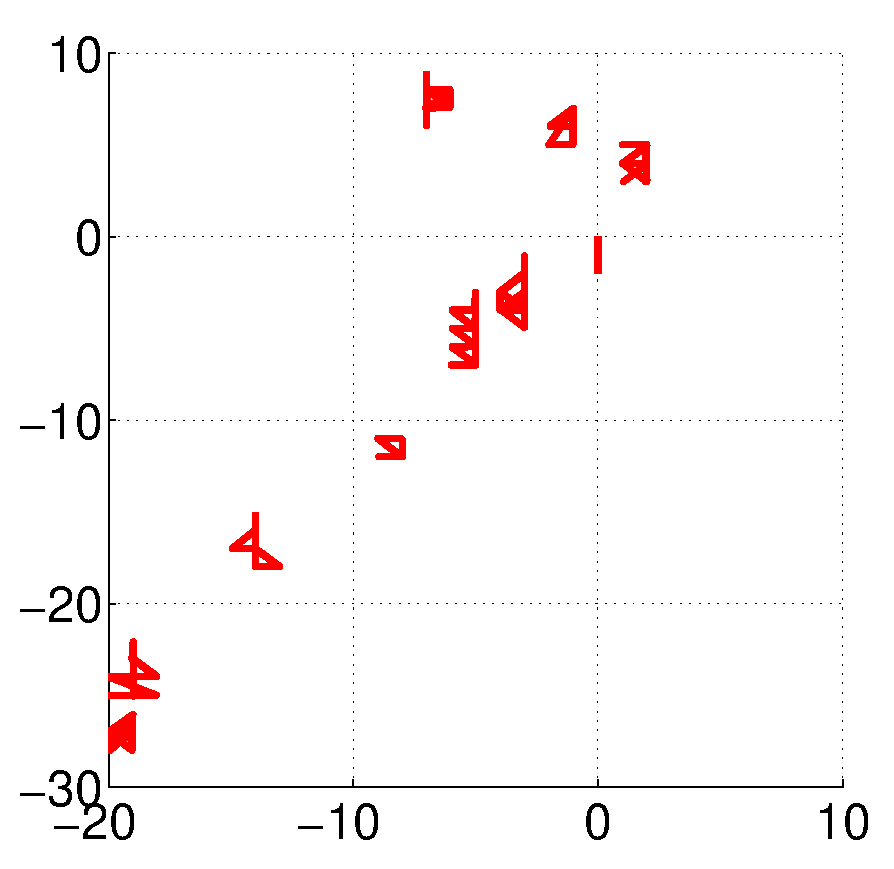
\includegraphics[width=30mm]{Figure/LeftEyeOpenLoop.eps}}  & \hspace{0.1cm} &
	  \parbox{30mm}{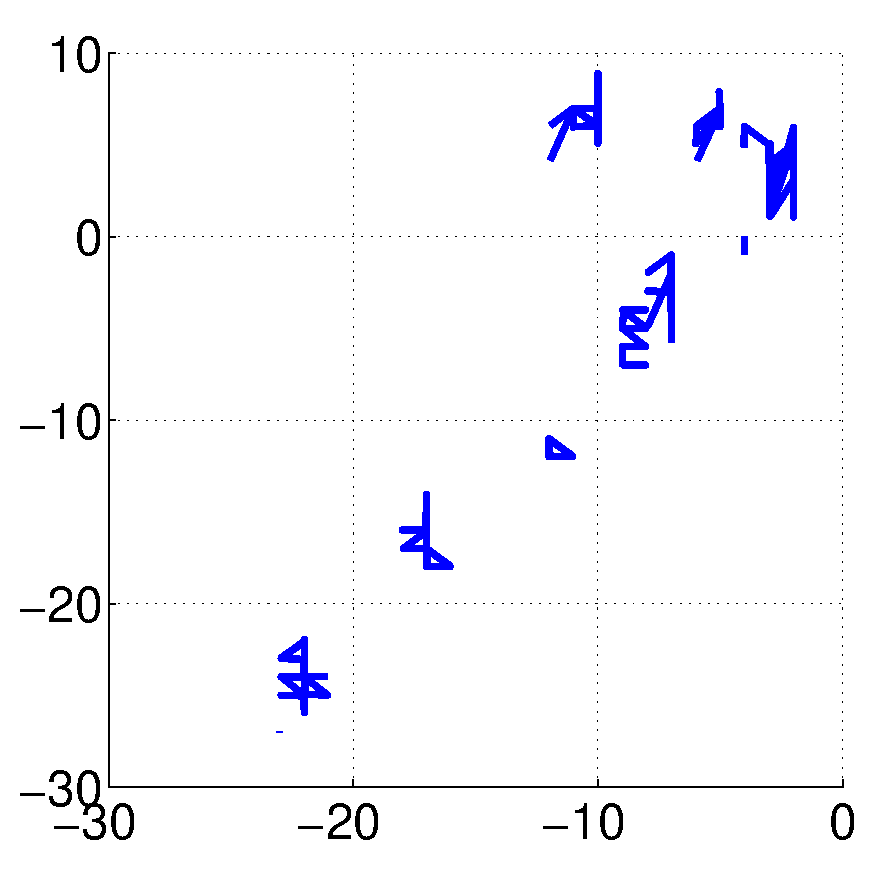
\includegraphics[width=30mm]{Figure/RightEyeOpenLoop.eps}}
	  \\
	  \parbox{30mm}{\centering Left eye } & \hspace{0.1cm} & \parbox{30mm}{\centering Right eye }
	  %	  \end{t\\
	  %	Top view & & Lateral view
  \end{tabular}
\end{center}
\caption{Open loop image plane errors $\uhand$ for different
choices of the redundant variable $q_{20}$. On the horizontal axis 
$u_r$ and $u_l$; vertical axis $v_r$ and $v_l$ (always in pixels).
The hand position in the image plane is represented 
by the small circles.  Each circle corresponds to a different open loop movement, i.e. a different value of $q_{20}$.
}\label{Fig:ImagePlaneOpenLoopErrors}
 \end{figure}

\subsection{Closed Loop}

The residual image plane errors 
due to imperfections in the forward kinematic model can be reduced by a visual closed loop
control strategy (\ref{Eq:ClosedLoopStrategy}), started immediately after the open loop phase. Relatively weak conditions on the learned 
Jacobian \cite{Samson91robot} guarantee the convergence of the image plane errors $\uhand$ to zero, and therefore
the convergence of the hand $\xhand$ on the target $\xtarget$. Figures
\ref{Fig:ImagePlaneClosedLoopErrors}, %\ref{Fig:TimeResponseClosedLoopErrors}, 
\ref{Fig:TimeResponseOpenClosedLoopErrors} and \ref{Fig:TimeResponseOpenClosedLoop}  
show how the hand is actually driven to the 
exact image center in both the image planes. The closed loop controller 
improves the accuracy of the reaching movement, but at the cost of a slower 
execution speed (see Figure \ref{Fig:TimeResponseOpenClosedLoop}); faster
executions couldn't be obtained by increasing the control loop gains, due to
the frame rate (thirty milliseconds) and the delays in the visual processing (hand localization and tracking).
Finally, it is important to notice 
the quasi-linearity of the path followed by the hand 
(see Figure \ref{Fig:ImagePlaneClosedLoopErrors}). This linearity denotes 
a good accuracy of the learned Jacobian.

\begin{figure}[th!]
  % Requires \usepackage{graphicx}
  \begin{center}
	\begin{tabular}{ccc}
	  \parbox{30mm}{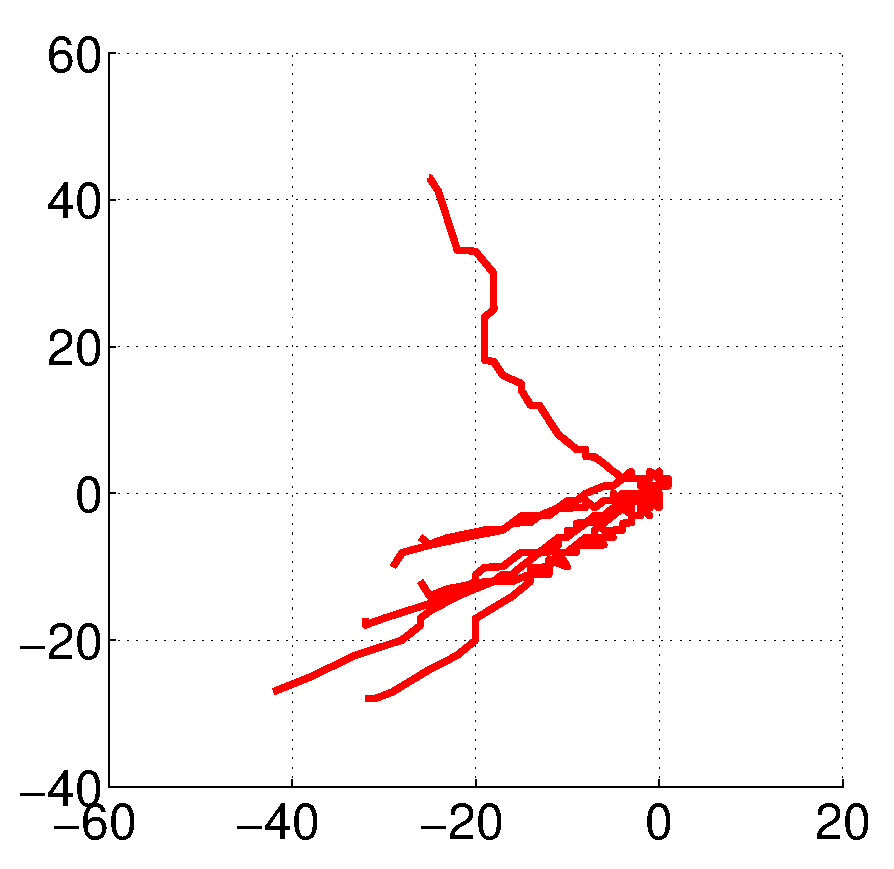
\includegraphics[width=30mm]{Figure/LeftEyeClosedLoop.eps}}  & \hspace{.1cm} &
	  \parbox{30mm}{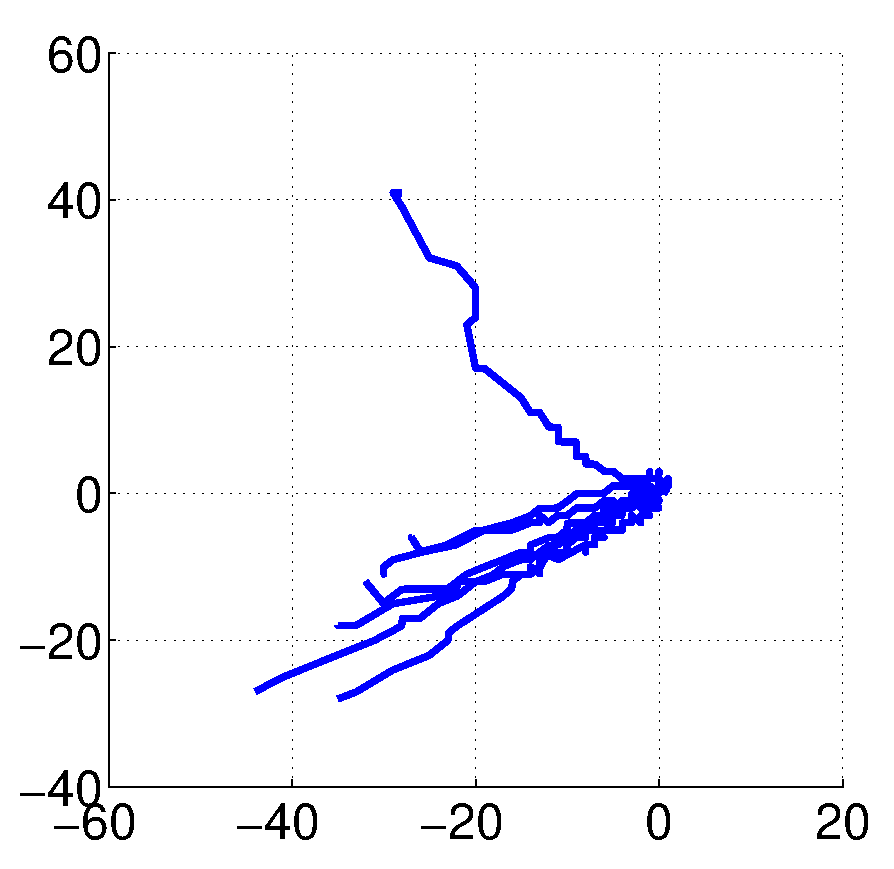
\includegraphics[width=30mm]{Figure/RightEyeClosedLoop.eps}}
	  \\
	  \parbox{30mm}{\centering Left eye } & \hspace{0.1cm} & \parbox{30mm}{\centering Right eye }
	  %	  \end{t\\
	  %	Top view & & Lateral view
  \end{tabular}
\end{center}
\caption{Traces of different closed loop control actions. Each trace correspond to a different Cartesian position of the target to be reached (which 
is always at the center of the image planes). All the traces end up in the image center thus indicating that the visual errors are completely eliminated by the closed loop controller.}\label{Fig:ImagePlaneClosedLoopErrors}
  \end{figure}

%\begin{figure}
%  % Requires \usepackage{graphicx}
%  \begin{center}
%	\begin{tabular}{ccc}
%	  \parbox{30mm}{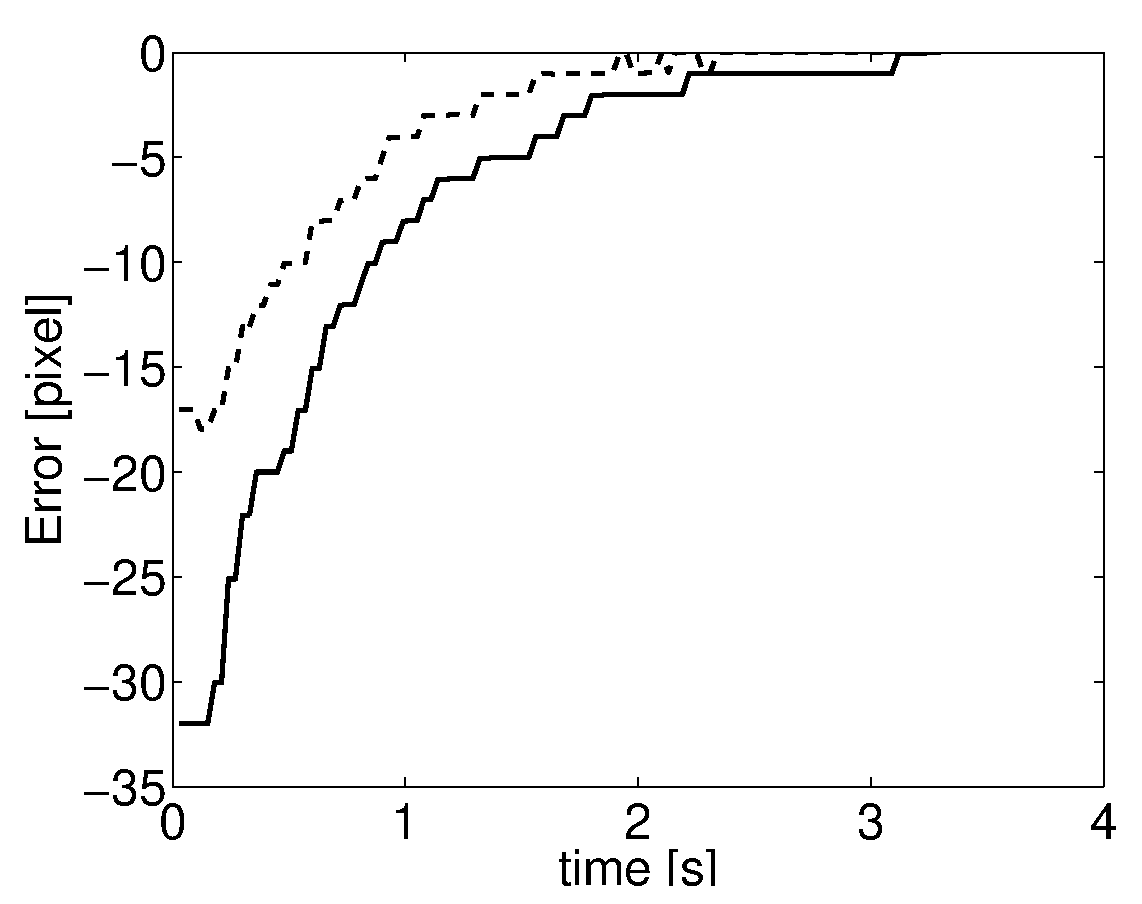
\includegraphics[width=30mm]{Figure/TimeReponseLeftClosedLoop.eps}}  & \hspace{.1cm} &
%	  \parbox{30mm}{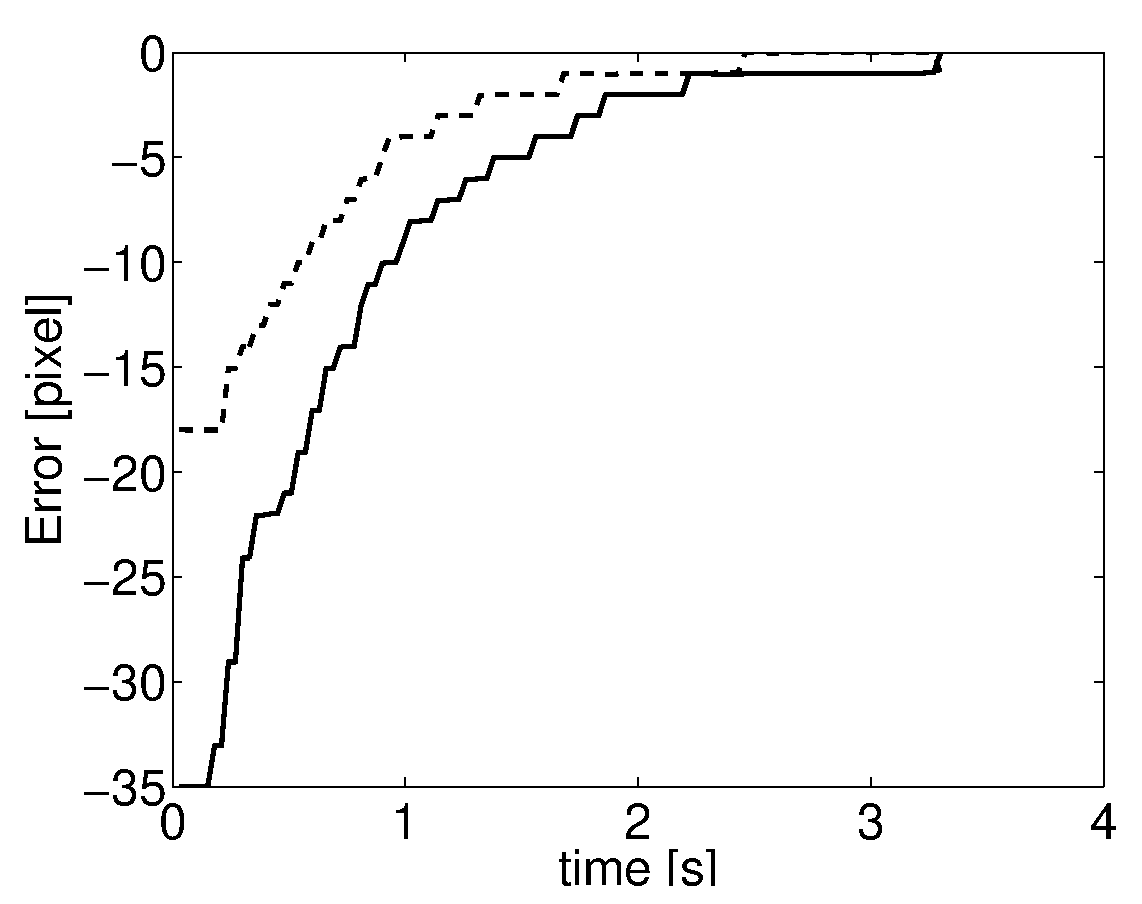
\includegraphics[width=30mm]{Figure/TimeReponseRightClosedLoop.eps}}
%	  \\
%	  \parbox{30mm}{\centering Left eye } & \hspace{0.1cm} & \parbox{30mm}{\centering Right eye }
%	  %	  \end{t\\
%	  %	Top view & & Lateral view
%  \end{tabular}
%\end{center}
%\caption{Time response of the closed loop controller. Solid lines: hand horizontal position in the left ($u_l$) and right ($u_r$). Dashed lines: vertical position, $v_l$ and $v_r$.}\label{Fig:TimeResponseClosedLoopErrors}
%  \end{figure}


\begin{figure}[th!]
  % Requires \usepackage{graphicx}
  \begin{center}
	\begin{tabular}{ccc}
	  \parbox{30mm}{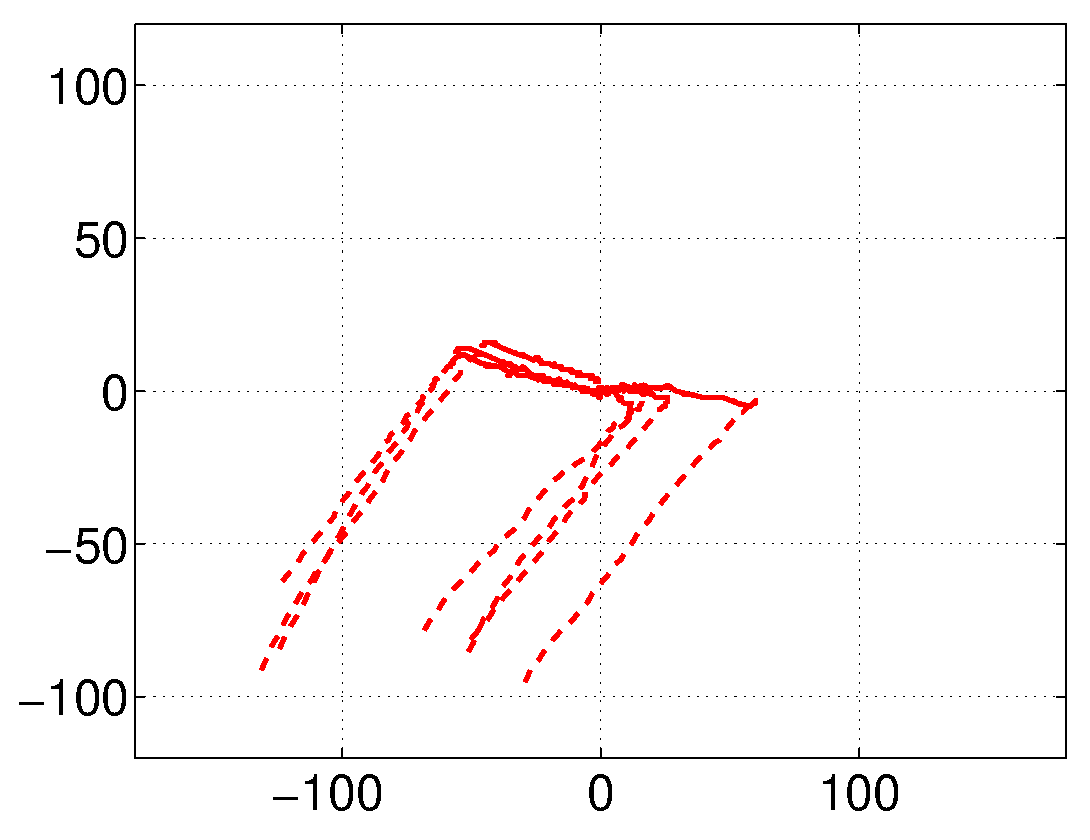
\includegraphics[width=30mm]{Figure/LeftEyeOpenClosedLoop.eps}}  & \hspace{.1cm} &
	  \parbox{30mm}{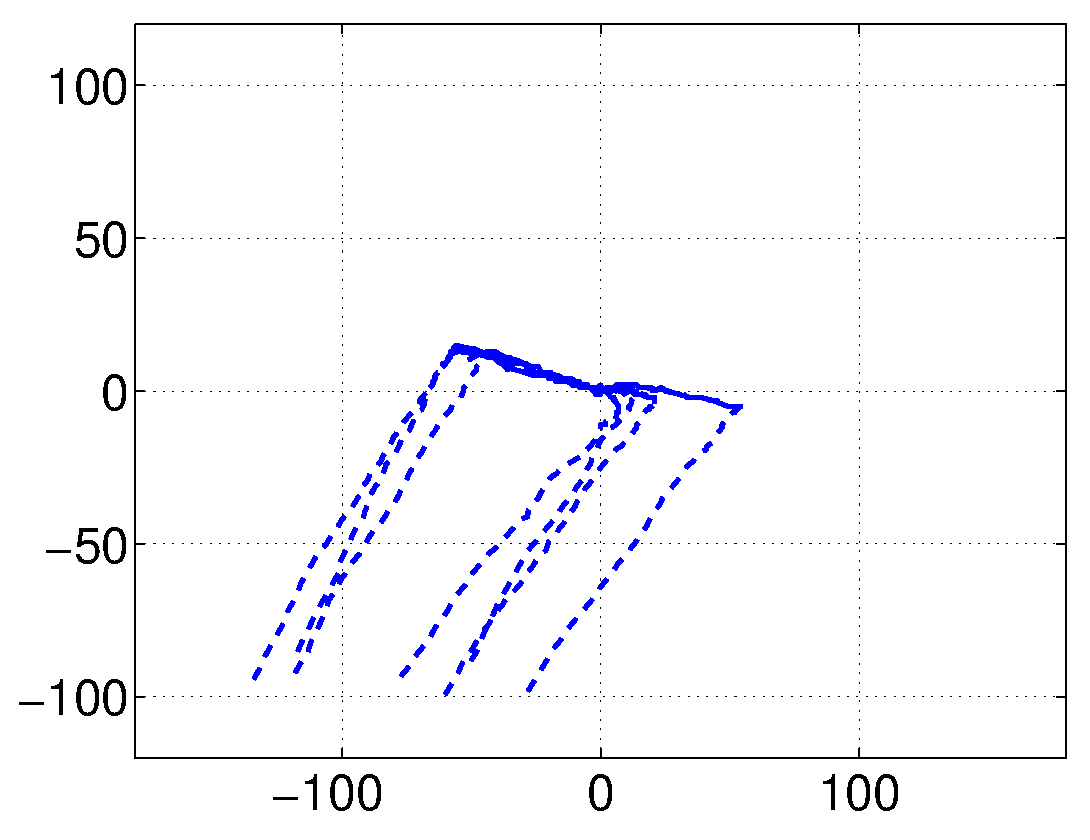
\includegraphics[width=30mm]{Figure/RightEyeOpenClosedLoop.eps}}
	  \\
	  \parbox{30mm}{\centering Left eye } & \hspace{.1cm} & \parbox{30mm}{\centering Right eye }
	  %	  \end{t\\
	  %	Top view & & Lateral view
  \end{tabular}
\end{center}
\caption{Movement of the hand on the image planes (320$\times$240)
during the execution of different reaching actions. 
Solid line: closed loop. Dashed trace: open loop. Clearly the open loop movement drives the hand to the target (the image centers) with a 
relatively small error. The closed loop phase reduces this error to zero.}\label{Fig:TimeResponseOpenClosedLoopErrors}
  \end{figure}
  
  \begin{figure}[th!]
  % Requires \usepackage{graphicx}
  \begin{center}
	\begin{tabular}{ccc}
	  \parbox{30mm}{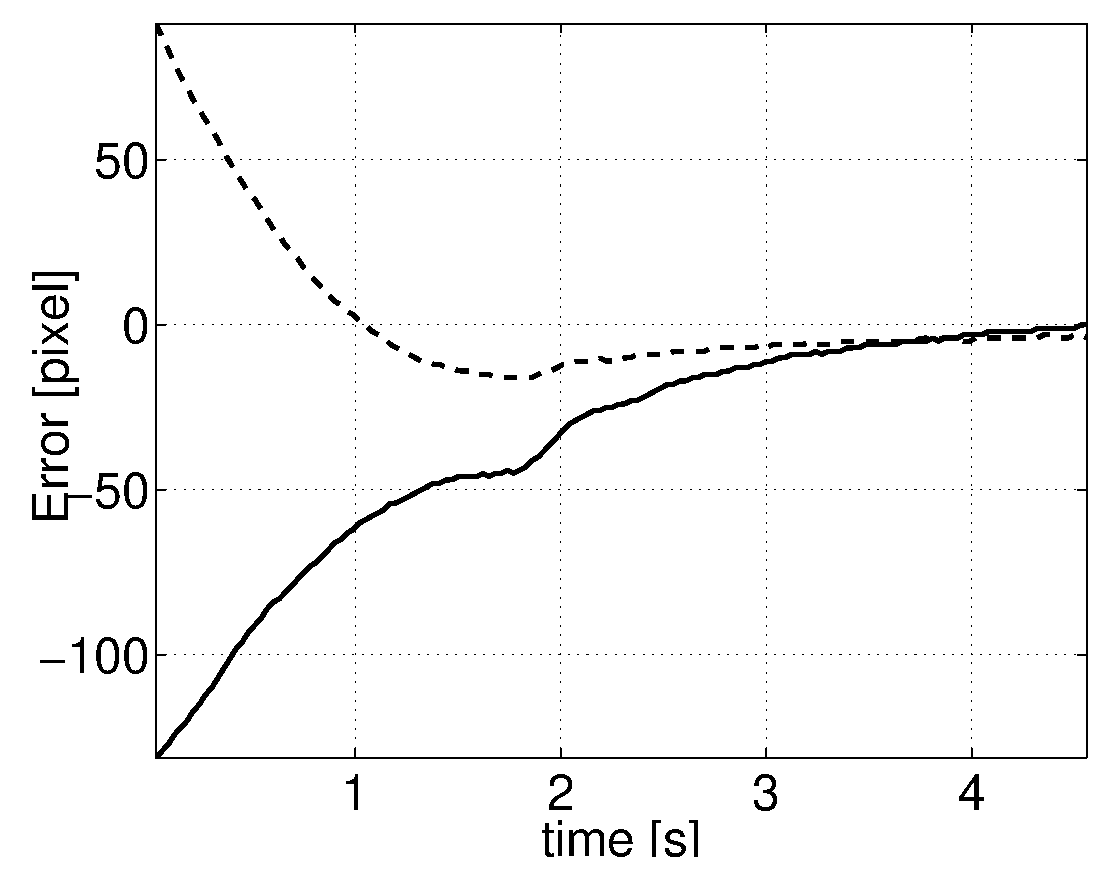
\includegraphics[width=30mm]{Figure/LeftEyeOpenClosedLoopTimeResponse.eps}}  & \hspace{.1cm} &
	  \parbox{30mm}{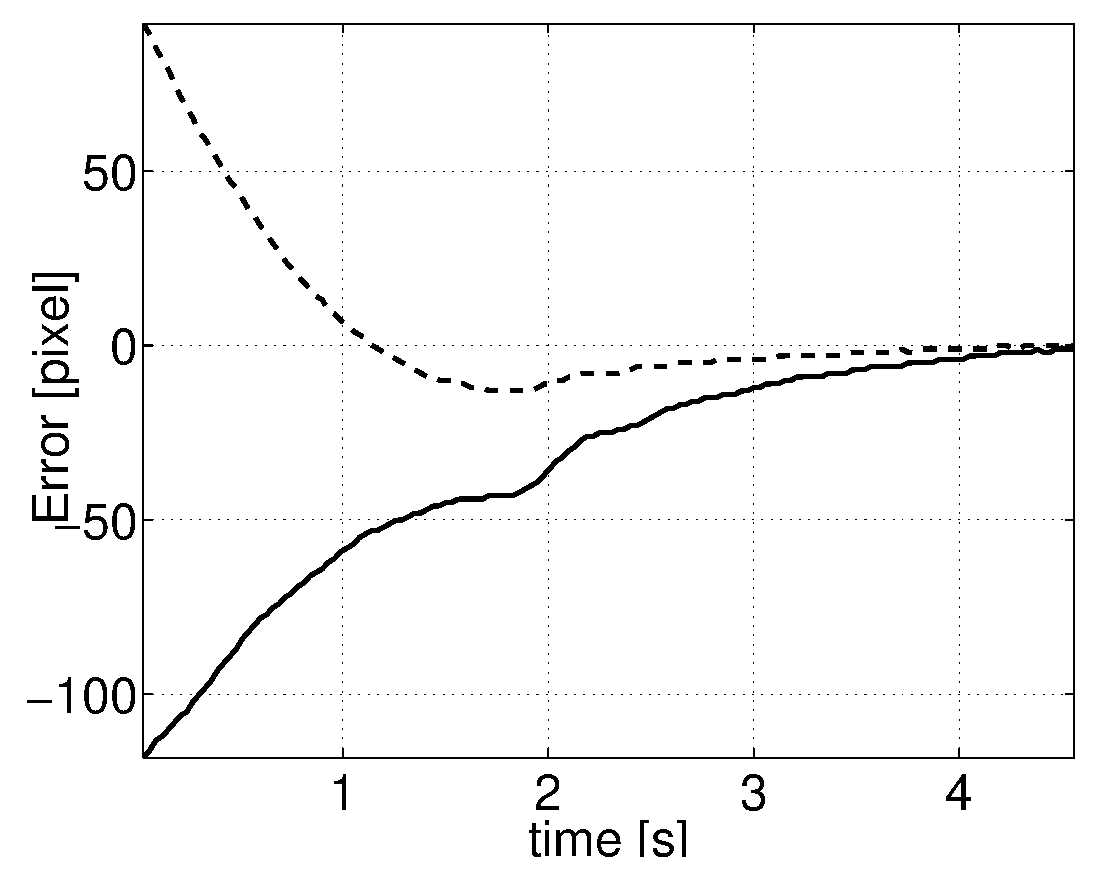
\includegraphics[width=30mm]{Figure/RightEyeOpenClosedLoopTimeResponse.eps}}
	  \\
	  \parbox{30mm}{\centering Left eye } & \hspace{.1cm} & \parbox{50mm}{\centering Right eye }
	  %	  \end{t\\
	  %	Top view & & Lateral view
  \end{tabular}
\end{center}
\caption{Time response of the closed loop and open loop strategy. Solid lines: $u_r$ and $u_l$. Dashed lines: $v_r$ and $v_l$. Remarkably, the open loop phase is faster but does not drive the hand exactly on the target. The closed loop is slower but more accurate.}\label{Fig:TimeResponseOpenClosedLoop}
\end{figure}


\subsection{Superimposed Open and Closed Loop}

Finally, we tested an alternative control strategy based on activating the closed loop 
phase immediately after the hand becomes visible on both image planes. This second strategy
is such that the open a closed loop strategies will be active at the same time for a 
certain amount of time. 
\newpage 
The structure is based on a classical control scheme, which can be represented as follows:

\begin{figure}[th!]
\begin{center}
\includegraphics[scale = 0.25]{Figure/OpenVSClosedLoop.eps}
\end{center}
\end{figure}

Practically, the feedforward control corresponds to the open loop part of the reaching movement.
It is activated exactly as described in Section \ref{sec:openReaching} and therefore it does not
require the hand to be visible in the image plane. The feedback control
instead corresponds to the closed loop part of the movement and can be activated when the hand
has been localized in both the image planes. Practically, the final solution can be described by the 
following scheme:

\begin{figure}[th!]
\begin{center}
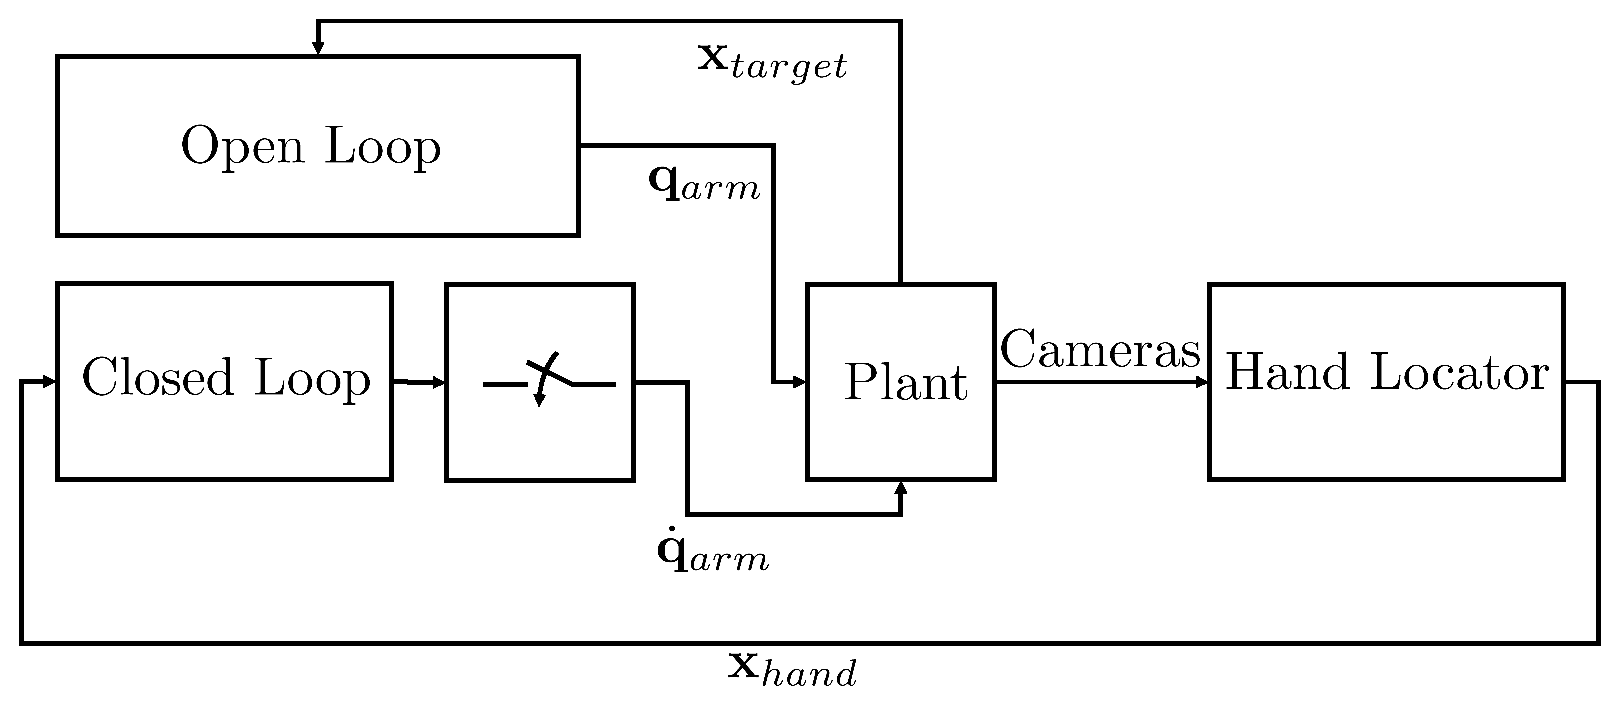
\includegraphics[scale = 0.25]{Figure/OpenVSClosedLoopSwitch.eps}
\end{center}
\end{figure}

Clearly, when both the open and closed loop controllers are active, the system receives position 
and velocity control simultaneously\footnote{A position command ${\mathbf q}_{arm,d}$ is 
always translated into a trajectory following command by moving 
the hand along a trajectory $\mathbf q_{arm}(t)$, $t \in [0, T]$ such that: $T$ is the execution time,
$\mathbf q_{arm}(0)$ is the arm position when the command is received, $\mathbf q_{arm}(T) = {\mathbf q}_{arm,d}$
is the desired final position, $\dot {\mathbf q}_{arm}(t) = 0$, $ \forall t > T$. If a velocity command $\dot {\mathbf q}_{arm,d}$ is received while executing a position
command $\mathbf q_{arm}(t)$, the original velocity command is transformed into a new one, nominally
$\dot {\mathbf q}_{arm} = \dot {\mathbf q}_{arm}(t) + \dot {\mathbf q}_{arm, d}$.}. 

A comparison between this control strategy and the one proposed in Section \ref{Eq:ClosedLoop}
is given in Figure \ref{Fig:TimeResponseOpenVSClosedLoopErrors} and \ref{Fig:TimeResponseOpenVSClosedLoop}. 
The second control strategy clearly outperforms the first one. As a matter of fact, the image plane movement (Figure \ref{Fig:TimeResponseOpenVSClosedLoopErrors})
is much more regular resulting in a unique linear movement instead of begin divided into two segments. Secondly, the
execution time is clearly reduced as it can be noted in Figure \ref{Fig:TimeResponseOpenVSClosedLoop}.


\begin{figure}
  % Requires \usepackage{graphicx}
  \begin{center}
	\begin{tabular}{ccc}
	  \parbox{30mm}{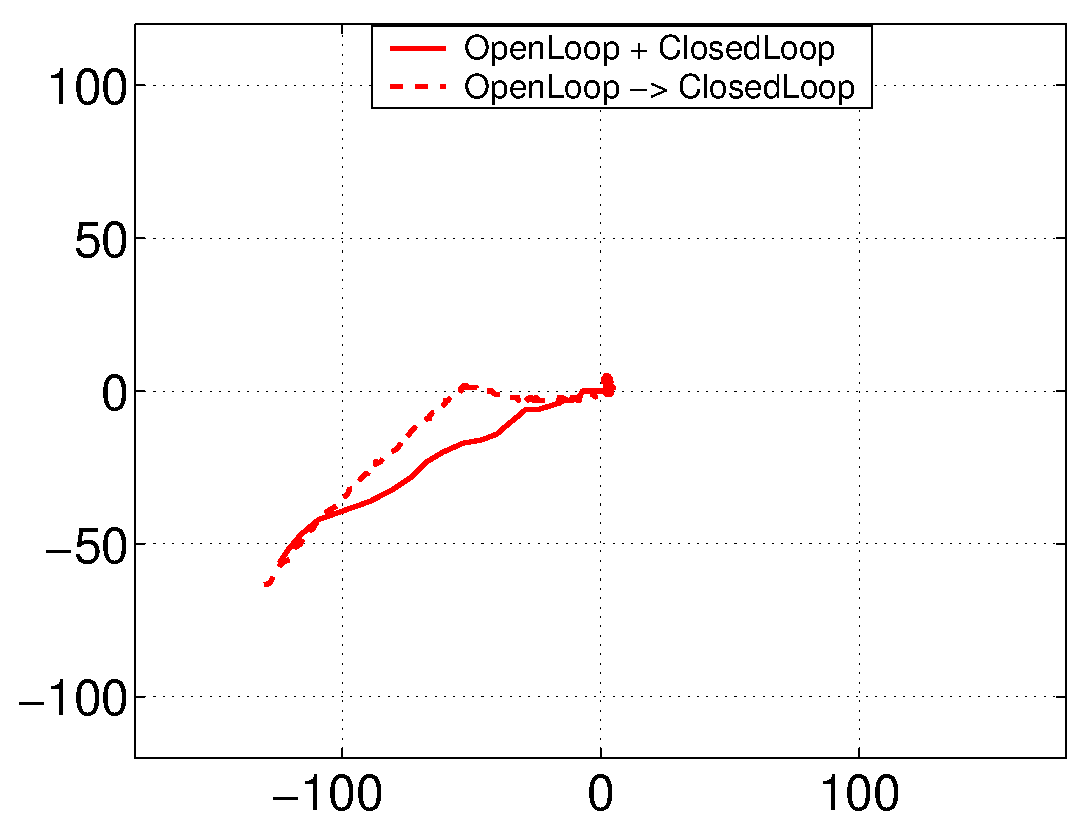
\includegraphics[width=30mm]{Figure/LeftEyeOpenVSClosedLoop.eps}}  & \hspace{.1cm} &
	  \parbox{30mm}{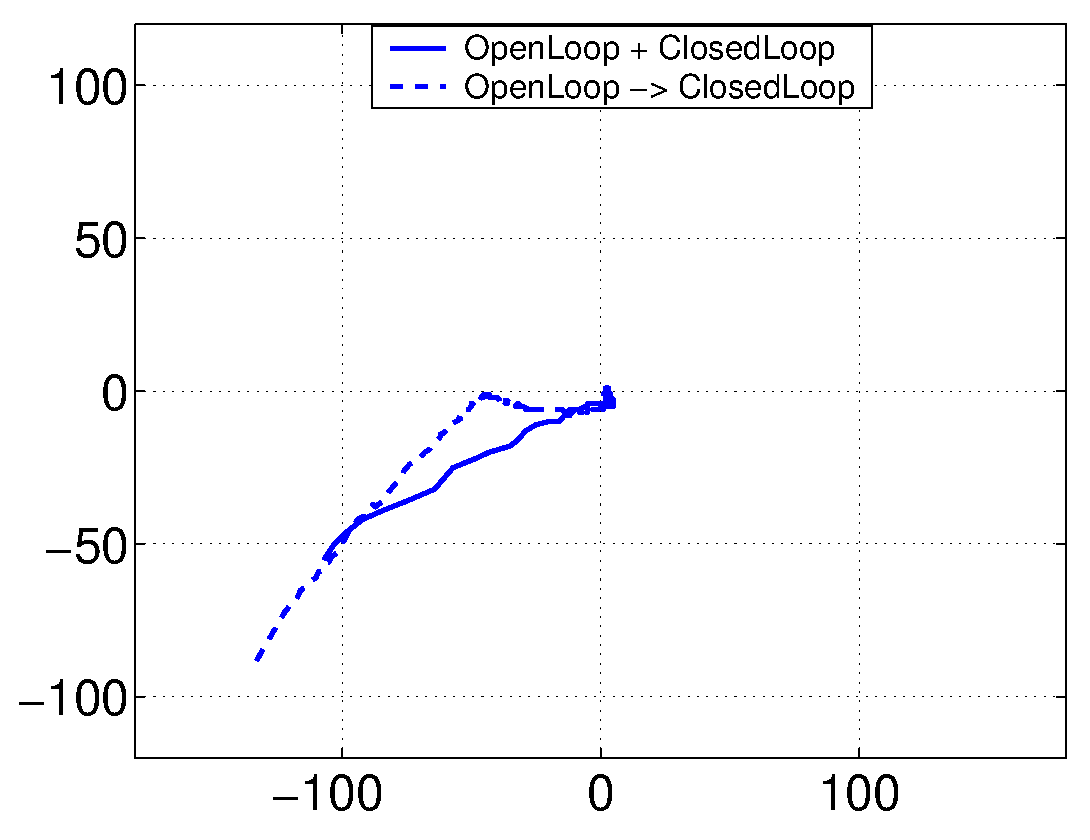
\includegraphics[width=30mm]{Figure/RightEyeOpenVSClosedLoop.eps}}
	  \\
	  \parbox{30mm}{\centering Left eye } & \hspace{.1cm} & \parbox{30mm}{\centering Right eye }
	  %	  \end{t\\
	  %	Top view & & Lateral view
  \end{tabular}
\end{center}
\caption{Movement of the hand on the image planes ($320 \times 240$)
during the execution of a single reaching movement. Dashed line: hand movement
during an open loop movement followed by a closed loop phase. Solid line: hand movement during 
the superposition of open and closed loop strategies.}\label{Fig:TimeResponseOpenVSClosedLoopErrors}
  \end{figure}
  
  \begin{figure}
  % Requires \usepackage{graphicx}
  \begin{center}
	  \parbox{40mm}{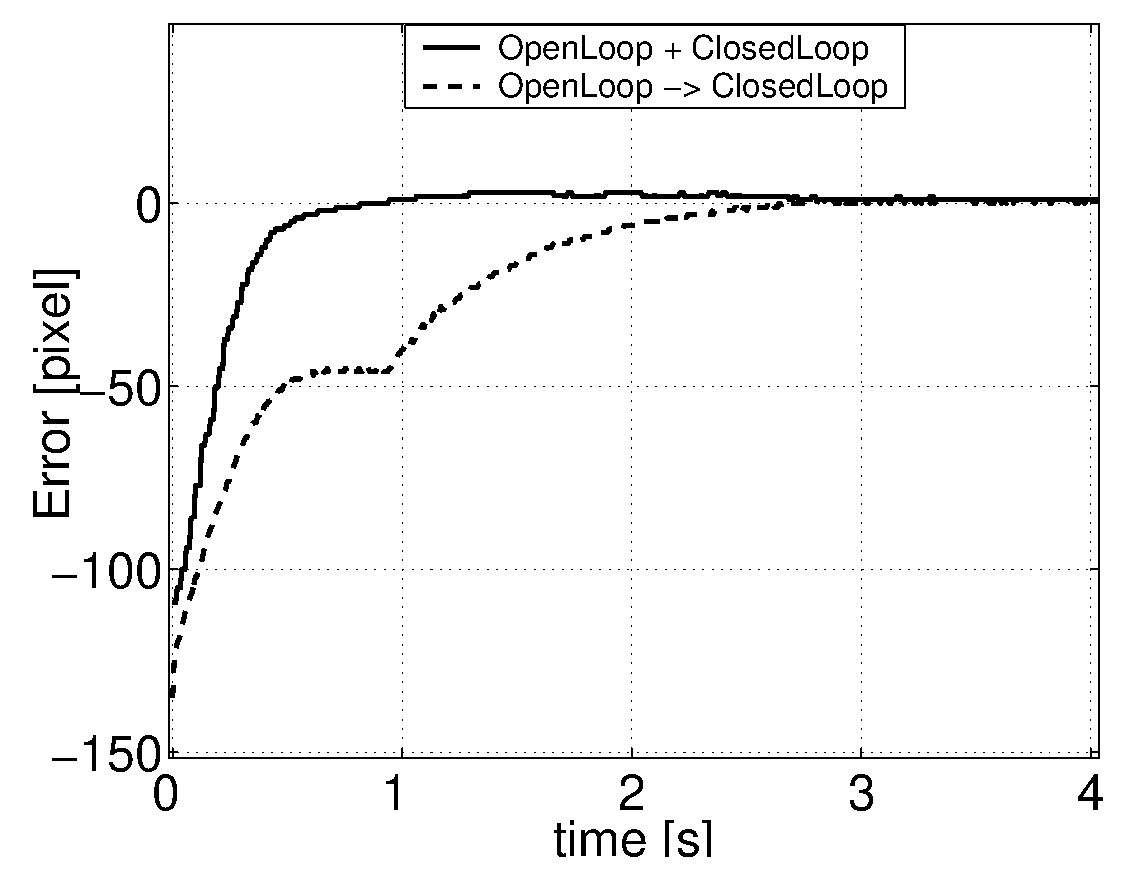
\includegraphics[width=40mm]{Figure/OpenVSClosedLoopTimeResponse1.eps}}
  \end{center}
\caption{Time response of the image plane position $u_l$. Dashed line: hand movement
during an open loop movement followed by a closed loop phase. Solid line: superposition of open and closed loop strategies.
 Remarkably, this second control architecture results in a faster response because when the hand becomes visible it is 
directly driven to the target without waiting for the open loop phase end.}\label{Fig:TimeResponseOpenVSClosedLoop}
  \end{figure}

\subsection{Null space movement}

In order to validate the quality of the Jacobian estimation, we tested the effects of a null space movement 
on the primary task (keeping $\uhand = 0$) as proposed in \cite{Mansard06jacobian}. A simple way to perform this testing is the following control strategy:
\begin{equation} \label{Eq:ClosedLoopStrategyRedundant}
\mathbf{\dot q}_{arm}=-k_1 \cdot \jacobian^\# \uhand + k_2 (I - \jacobian^\# \jacobian) \mathbf w, 
\end{equation}
where $I \in \mathbb R^{4 \times 4}$ is the identity matrix, $\mathbf w \neq 0$ is a 
randomly chosen vector in $\mathbb R^4$ and $k_1$, $k_2$ are positive constants. 
Ideally, the strategy (\ref{Eq:ClosedLoopStrategyRedundant}) should allow arm movements 
$\mathbf{q}_{arm} \neq 0$ while leaving the hand position $\uhand$ unperturbed. Practically we observed 
a minimal image plane movement (Figure \ref{Fig:RedundancyImagePlane})
as oppposed to a relatively large arm movement (Figure \ref{Fig:RedundancyArm}). These results 
further prove the quality of our Jacobian estimation.

\begin{figure}
  % Requires \usepackage{graphicx}
  \begin{center}
	\begin{tabular}{ccc}
	  \parbox{30mm}{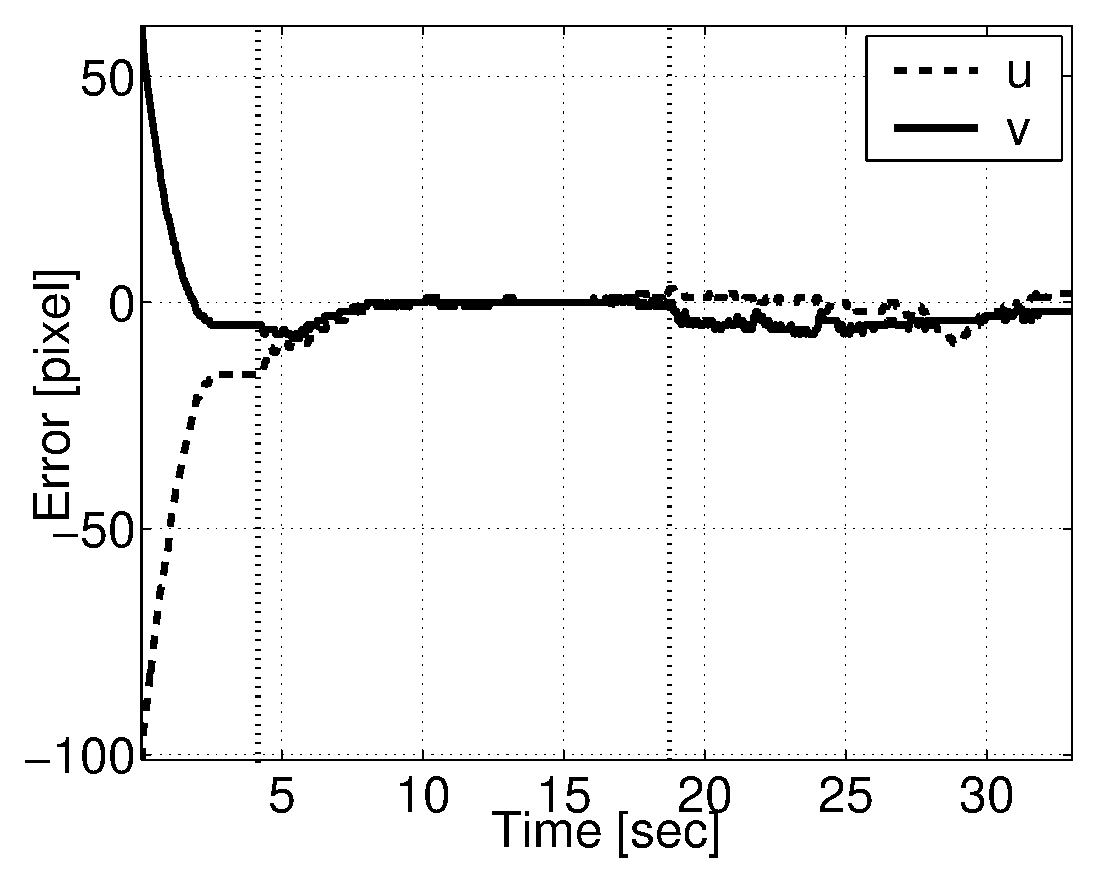
\includegraphics[width=30mm]{Figure/RedundancyLeft.eps}}  & \hspace{.1cm} &
	  \parbox{30mm}{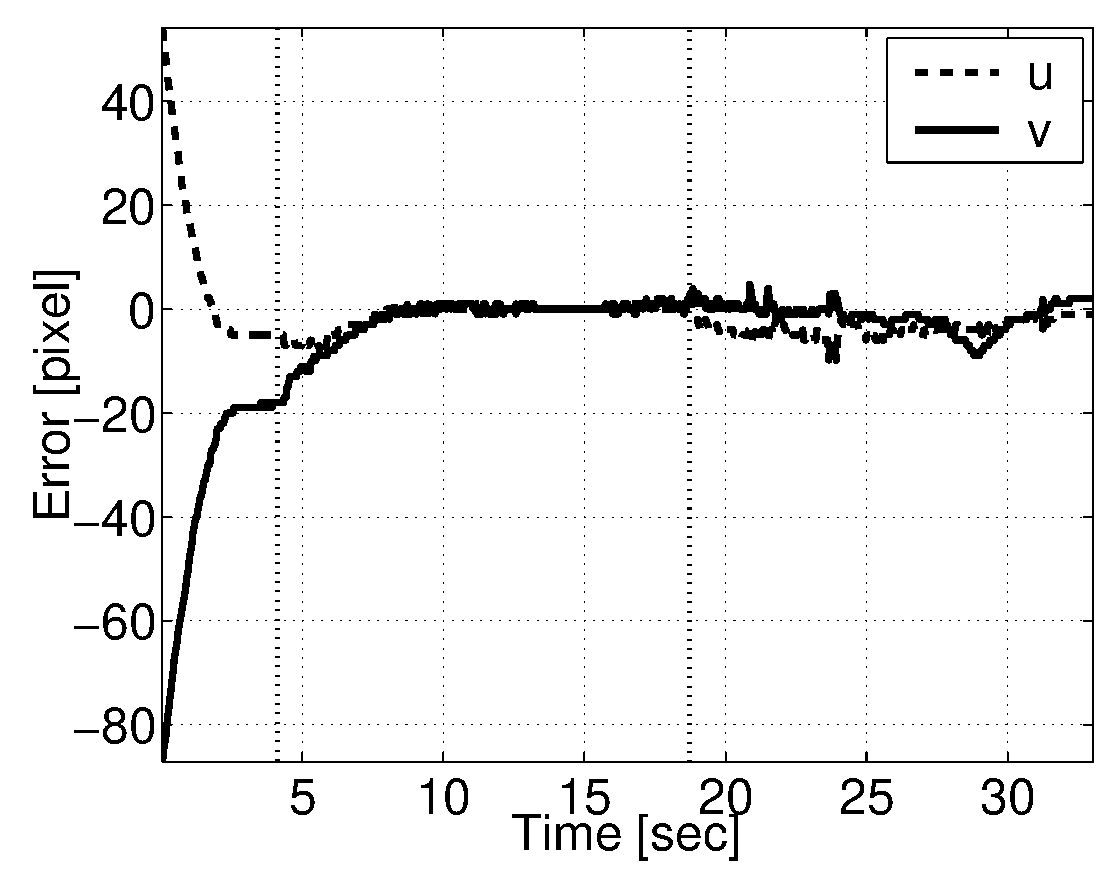
\includegraphics[width=30mm]{Figure/RedundancyRight.eps}}
	  \\
	  \parbox{30mm}{\centering Left eye } & \hspace{.1cm} & \parbox{30mm}{\centering Right eye }
	  %	  \end{t\\
	  %	Top view & & Lateral view
  \end{tabular}
\end{center}
\caption{Image plane movements during a three phase reaching. 
First the open loop, then the closed loop and finally a movement 
in the null space of the given task (keeping the hand in fixations). 
Each phase is delimited by a vertical dotted line.
}\label{Fig:RedundancyImagePlane}
  \end{figure}
  
  \begin{figure}
  % Requires \usepackage{graphicx}
  \begin{center}
	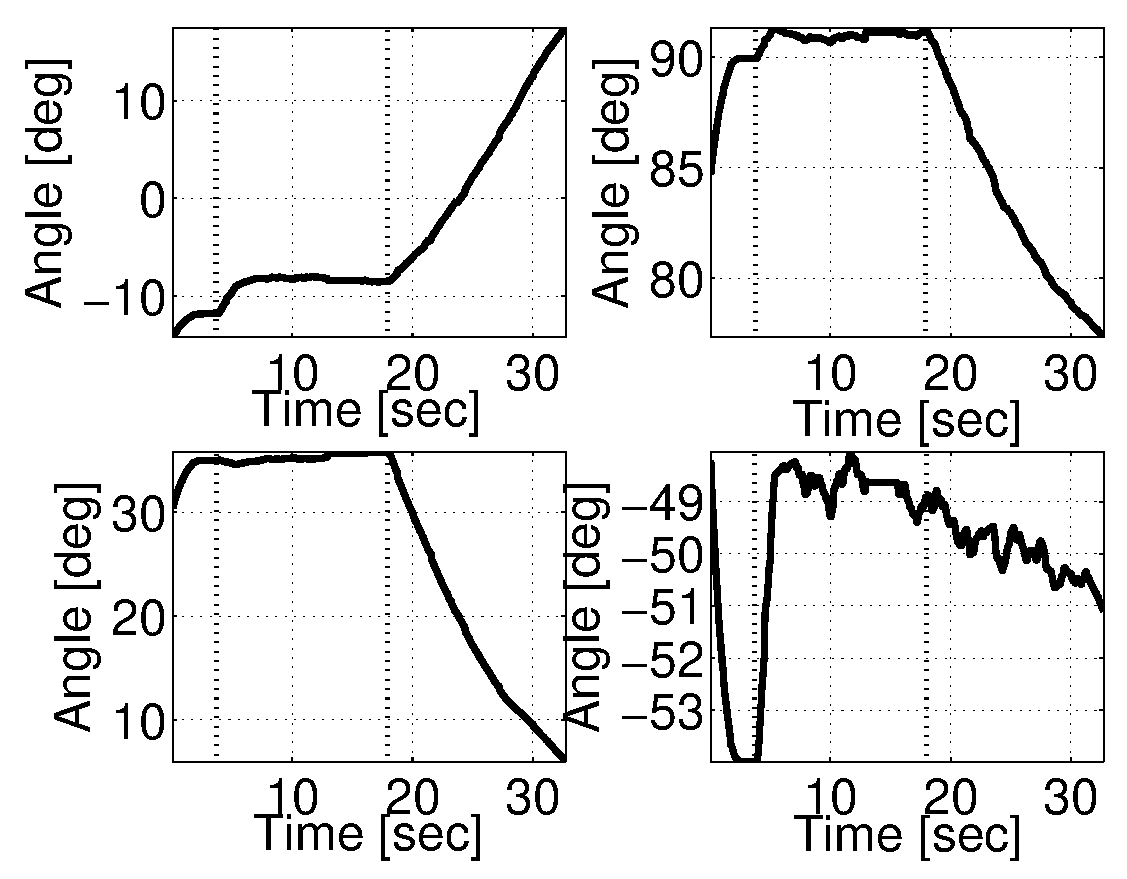
\includegraphics[width=60mm]{Figure/RedundancyArm.eps}
	\end{center}
\caption{Arm movement corresponding to the image plane movements shown in Figure \ref{Fig:RedundancyImagePlane}.
 Remarkably, the null space movement is characterized by large joint movements which are however not visible 
in the image plane due to the jacobian based compensation.} \label{Fig:RedundancyArm}
  \end{figure}
%\section{Conclusion}
future work:
stereovision, fourier for extracting frequencies so that also head can move. neural network to use. better use of bics.



% conference papers do not normally have an appendix

% use section* for acknowledgement
\section*{Acknowledgment}
% optional entry into table of contents (if used)
%\addcontentsline{toc}{section}{Acknowledgment}
The authors would like to thank...

% trigger a \newpage just before the given reference
% number - used to balance the columns on the last page
% adjust value as needed - may need to be readjusted if
% the document is modified later
%\IEEEtriggeratref{8}
% The "triggered" command can be changed if desired:
%\IEEEtriggercmd{\enlargethispage{-5in}}

% references section
% NOTE: BibTeX documentation can be easily obtained at:
% http://www.ctan.org/tex-archive/biblio/bibtex/contrib/doc/

% can use a bibliography generated by BibTeX as a .bbl file
% standard IEEE bibliography style from:
% http://www.ctan.org/tex-archive/macros/latex/contrib/supported/IEEEtran/bibtex
\bibliographystyle{IEEEtran}
% argument is your BibTeX string definitions and bibliography database(s)
%\bibliography{IEEEabrv,bib/paper}
\bibliography{bib/paper}
%
% <OR> manually copy in the resultant .bbl file
% set second argument of \begin to the number of references
% (used to reserve space for the reference number labels box)
%\begin{thebibliography}{1}

%\bibitem{IEEEhowto:kopka}
%H.~Kopka and P.~W. Daly, \emph{A Guide to {\LaTeX}}, 3rd~ed.\hskip 1em plus
%  0.5em minus 0.4em\relax Harlow, England: Addison-Wesley, 1999.
%@INPROCEEDINGS{JHRAUW06-12,
%  author = {Lorenzo Jamone and Giorgio Metta and Franscesco Nori and Giulio Sandini},
%  title = {James: A Humanoid Robot Acting over an Unstructured World},
%  booktitle = {6th IEEE-RAS International Conference on Humanoid Robots},
%  year = {2006},
%  pages = {143-150},
%  address = {Genova, Italy},
%  month = {December},
%  note = {Humanoids},
%  abstract = {The recent trend of humanoid robotics research has been deeply influenced
%	by concepts such as embodiment, embodied interaction and emergence.
%	In our view, these concepts, beside shaping the controller, should
%	guide the very design process of the modern humanoid robotic platforms.
%	In this paper, we discuss how these principles have been applied
%	to the design of a humanoid robot called James. James has been designed
%	by considering an object manipulation scenario and by explicitly
%	taking into account embodiment, interaction and the exploitation
%	of smart design solutions. The robot is equipped with moving eyes,
%	neck, arm and hand, and a rich set of sensors, enabling proprioceptive,
%	kinesthetic, tactile and visual sensing. A great deal of effort
%	has been devoted to the design of the hand and touch sensors. Experiments,
%	e.g. tactile object classification, have been performed, to validate
%	the quality of the robot perceptual capabilities.},
%  pdf = {G:\Science\james\JHRAUW06-12.pdf},
%  timestamp = {2007.03.10},
%  url = {http://www.robotcub.org/misc/review2/06_Jamone_Metta_Nori_Sandini.pdf}
%}
%
%\end{thebibliography}
%

% that's all folks
\end{document}


